\documentclass[letterpaper, 11pt, oneside]{book}

\usepackage{style}  % If you feel like procrastinating, mess with this file
\usepackage{algo}   % Thank you Jeff, very cool!
\usepackage{quiver} % https://q.uiver.app/

\addbibresource{refs.bib}

% Required reading
% https://jmlr.csail.mit.edu/reviewing-papers/knuth_mathematical_writing.pdf
%   Along with required viewing:
%   https://www.youtube.com/watch?v=N6QEgbPWUrg&list=PLOdeqCXq1tXihn5KmyB2YTOqgxaUkcNYG
% https://faculty.math.illinois.edu/~west/grammar.html

% % % % % % % % % %
%     Cursor      %
%     Parking     %
%     Lot         %
% % % % % % % % % %

% Disable check for mismatched parens/brackets/braces
%     chktex-file 9
% Disable check for different counts of parents/brackets/braces
%     chktex-file 17

\regtotcounter{figure}

\title{\vspace{-100pt}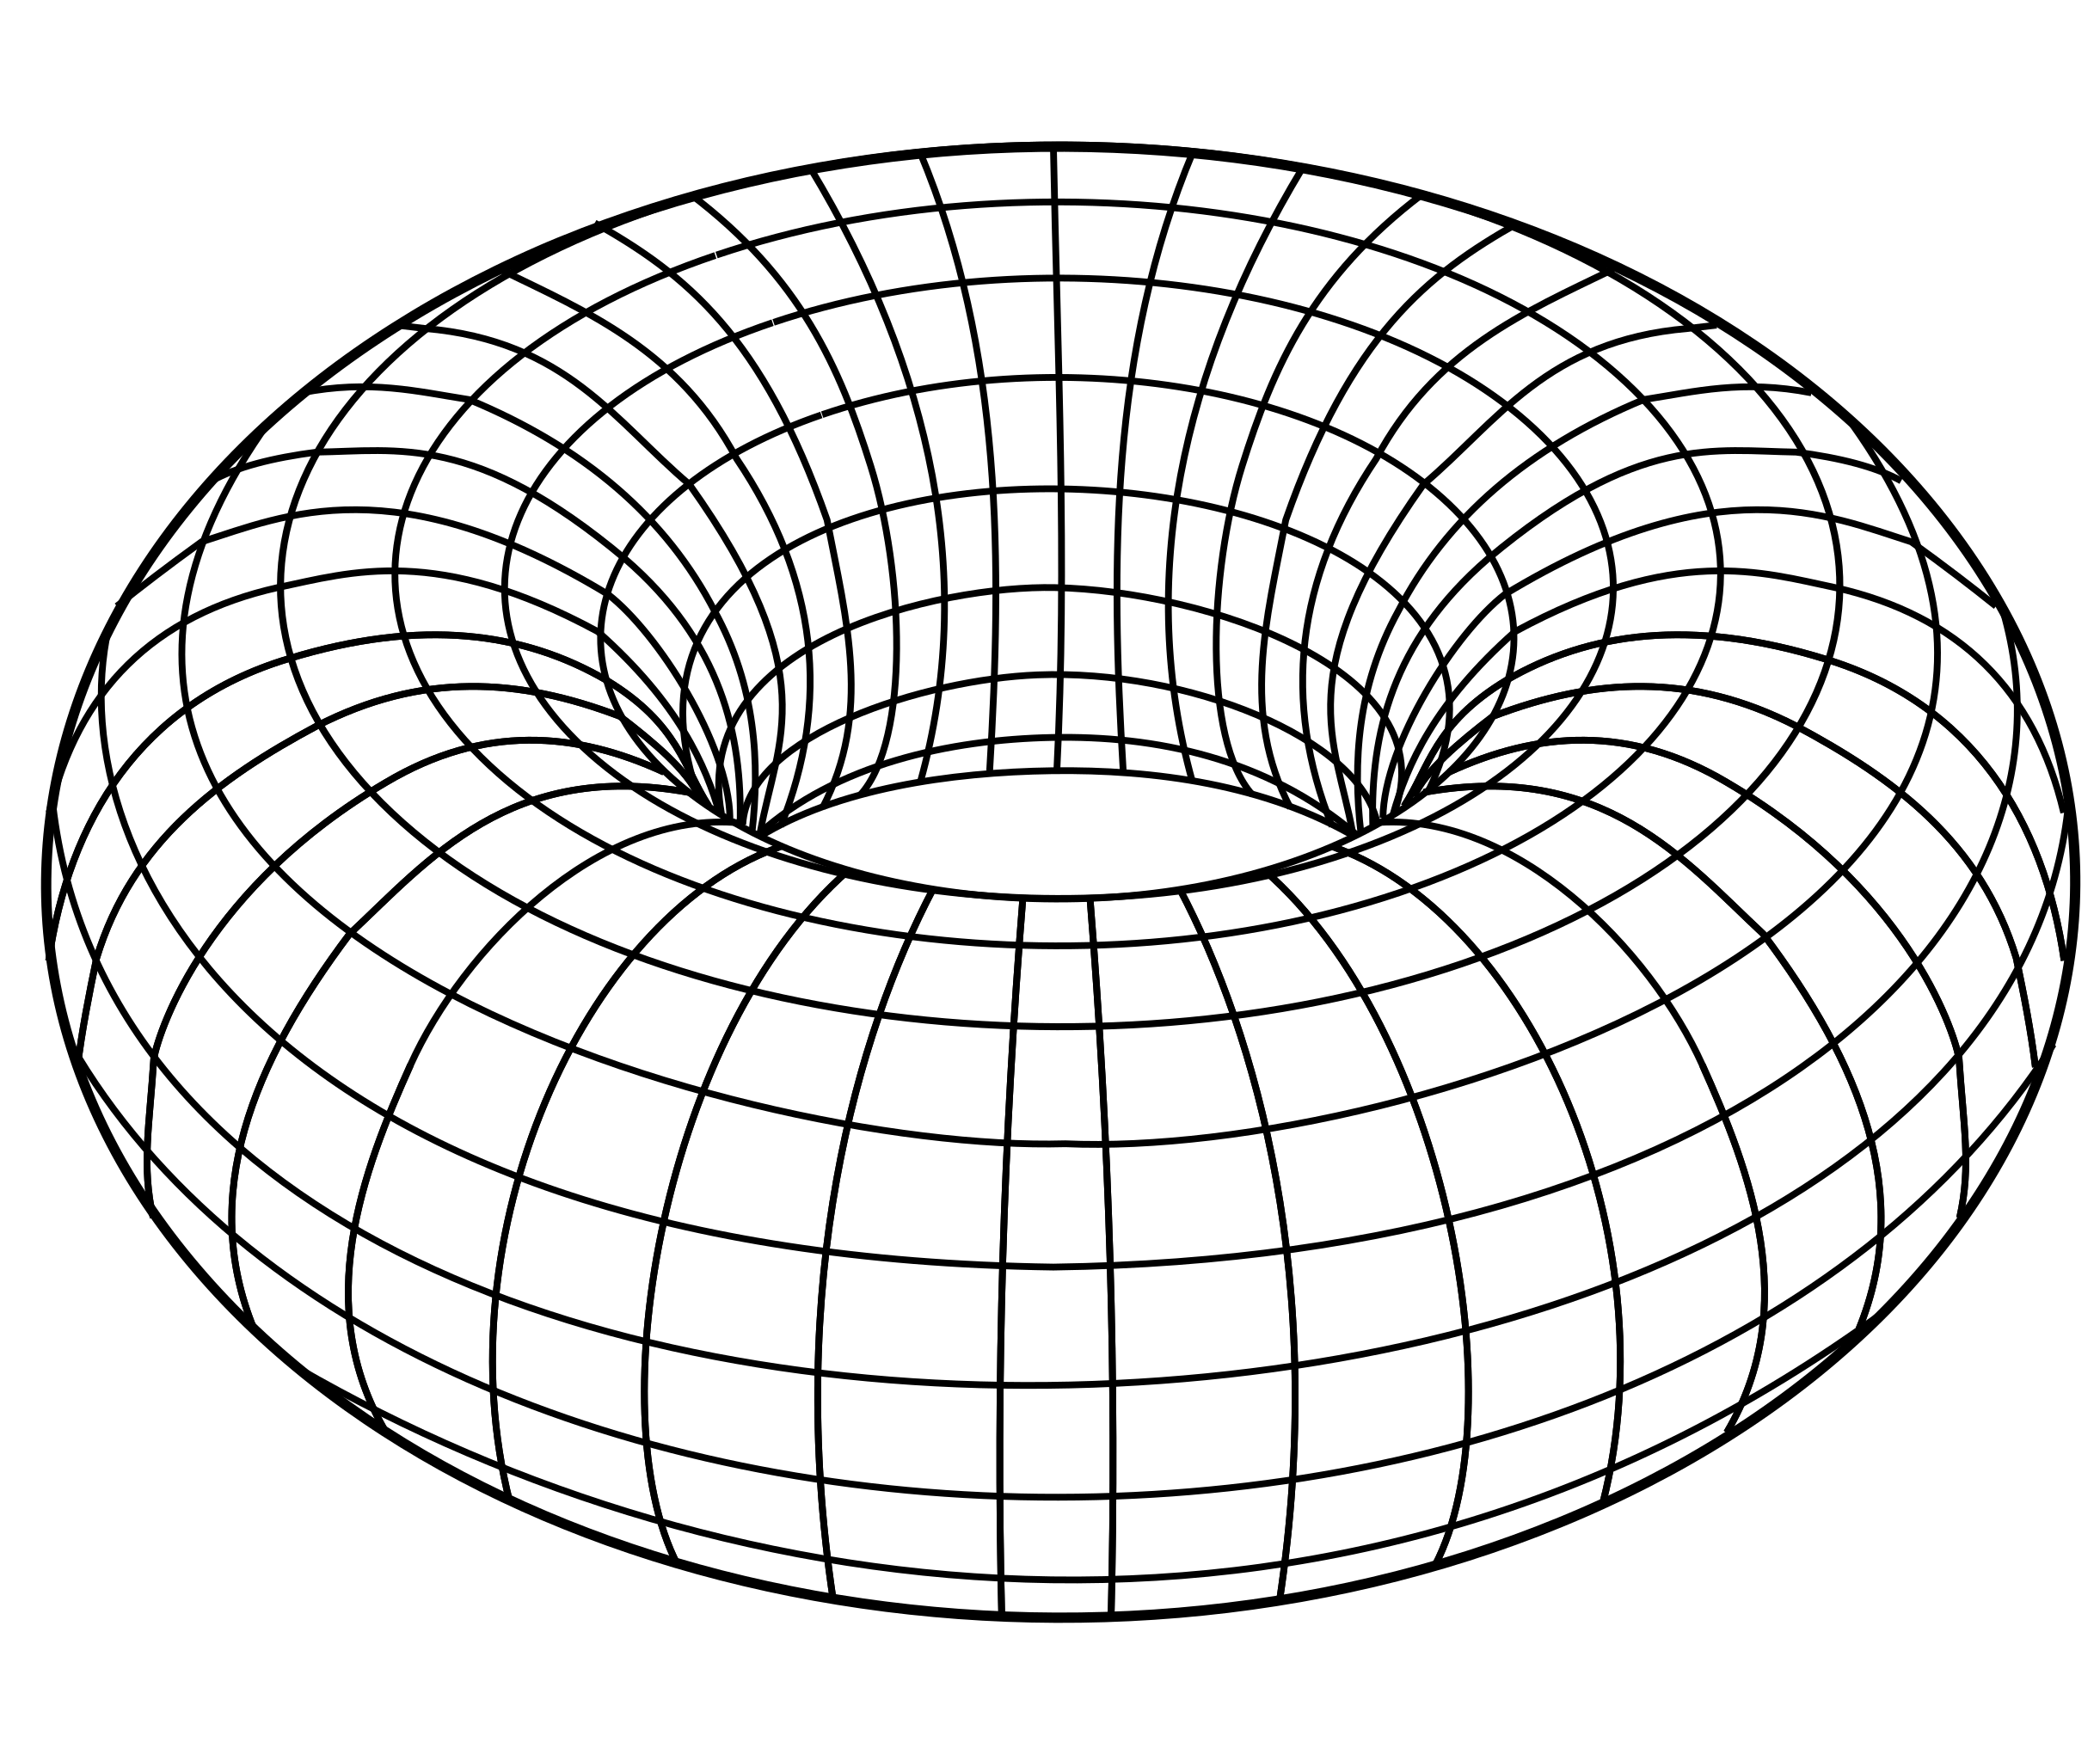
\includegraphics[width=0.75\textwidth]{figs/title.png} \\ {\Huge Topology Notes and Exercises} \\ {\small With $\total{figure}$ Figures}}
\nocite{title_pic}
\author{\Large Anakin Dey}
\DTMsavenow{now}
\date{\small Last Edited on \today\ at \DTMfetchhour{now}:\DTMfetchminute{now}}

\begin{document}
\frontmatter
\maketitle

\section*{TODOs}

\quest{Change the style of enumerates from ``1.'' to ``(1)''}

\quest{Proper Exercise Header}

\quest{Proper Chapter Header}

\quest{Table of Contents}

\quest{Named Theorem List}

\quest{Many TODOs within proofs throughout}

\tableofcontents
\clearpage


\listoftheorems[ignoreall, show={defn}, title={List of Definitions}]

\listoftheorems[ignoreall, show={ex}, title={List of Examples and Counterexamples}]

\mainmatter

\chapter{Metric Spaces}

The most familiar example of a metric space is $\R^{n}$ with $\dist(x, y) = \pqty{\sum_{i = 1}^{n} (x_{i} - y_{i})^{2}}^{1/2}$.
We also have a notion of continuity.
A function $f$ is \emph{continuous at a point $x$} if for all $\e > 0$, there exists $\delta > 0$ such that $\dist(x, y) < \delta \implies \dist(f(x), f(y)) < \e$.
We wish to generalize this notion.

\begin{defn}[Metric Spaces]
  A \emph{metric space} is a set $X$ equipped with a distance function $\dist\colon X \times X \to \R$ called a \emph{metric} satisfying
  \begin{enumerate}
    \item $\dist(x, y) \geq 0$ with equality if and only if $x = y$
    \item $\dist(x. y) = \dist(y, x)$
    \item $\dist(x, z) \leq \dist(x, y) + \dist(y, z)$.
  \end{enumerate}
\end{defn}

\begin{defn}[$\e$-ball]
  For a point $x$ in some metric space $X$, the \emph{$\e$-ball about x} is
  \[
    B_{\e}(x) \defeq \set{y \in X | \dist(x, y) < \e}.
  \]
\end{defn}

It is not hard to rephrase the definition of continuity in terms of $\e$-balls.

\begin{defn}[Open and Closed Sets in $\R$]
  A subset $U$ of some metric space $X$ is \emph{open} if for all $x \in U$ there exists $\e > 0$ such that $B_{\e}(x) \subseteq U$.
  A subset $C$ is \emph{closed} if its complement is open.
\end{defn}

We can actually even rephrase continuity in terms of open sets.

\clearpage

\begin{prop}
  A function $f\colon X \to Y$ between metric spaces is continuous if and only if $f^{-1}(U)$ is open for every open set $U \subseteq Y$.
\end{prop}
\begin{pf}
  Suppose $f\colon X \to Y$ is continuous.
  Let $U \subset Y$ be some open set and let $f(x) \in U$.
  Then there exists $\e > 0$ such that $B_{\e}(f(x)) \subseteq U$.
  By continuity of $f$, there exists $\delta > 0$ such that $f(B_{\delta}(x)) \subseteq B_{e}(f(x))$.
  Thus $B_{\delta}(x) \subseteq f^{-1}(U)$ and $f^{-1}(U)$ is open.

  Conversely, suppose that $f^{-1}(U)$ is open for any open $U \subseteq Y$.
  Let $\e > 0$.
  Then $B_{\e}(f(x))$ is open and $f^{-1}(B_{\e}(f(x)))$ is open and contains $x$.
  Thus there exists $\delta > 0$ such that $B_{\delta}(x) \subseteq f^{-1}(B_{\e}(f(x)))$.
  Thus $f(B_{\delta}(x)) \subseteq B_{\e}(f(x))$ and $f$ is continuous.
\end{pf}

This can also all be rephrased in terms of closed sets, rather than open sets.

\begin{ex}[Other Metrics on $\R$]
  We can also equip other metrics on $\R^{n}$.
  \begin{align*}
    \dist_{2}(x, y) &= \sum_{i = 1}^{n} \abs{x_{i} - y_{i}} \\
    \dist_{3}(x, y) &= \max_{i = 1}^{n} (\abs{x_{i} - y_{i}})
  \end{align*}
\end{ex}

However it turns out that for $\R^{n}$, choice between these 3 metrics is irrelevant.

\begin{prop}
  Suppose $\dist_{1}$ and $\dist_{2}$ are two metrics on the same set $X$ such that for any $x \in X$ and $\e > 0$, there exists $\delta > 0$ such that
  \[
    \dist_{1}(x, y) < \delta \implies \dist_{2}(x, y) < \e
  \]
  and
  \[
    \dist_{2}(x, y) < \delta \implies \dist_{1}(x, y) < \e.
  \]
  Then these metrics define the same open sets in $X$.
\end{prop}

\begin{pf}
  \quest{TODO:\@ PROOF}
\end{pf}

\begin{cor}
  The following metrics define the same open sets in $\R^{n}$:
  \begin{align*}
    \dist(x, y) &= \pqty{\sum_{i = 1}^{n} (x_{i} - y_{i})^{2}}^{1/2} \\
    \dist_{2}(x, y) &= \sum_{i = 1}^{n} \abs{x_{i} - y_{i}} \\
    \dist_{3}(x, y) &= \max_{i = 1}^{n} (\abs{x_{i} - y_{i}})
  \end{align*}
\end{cor}

\clearpage

\subsection*{Exercises}

\begin{exercise}[\tcite{book:Bredon} 1.1.1]
  Consider the set $X$ of all continuous real valued functions on $[0, 1]$.
  Show that
  \[
    \dist(f, g) = \int_{0}^{1} \abs{f(x) - g(x)} \dd{x}
  \]
  defines a metric on $X$.
  Is this still the case if continuity is weakened to integrability?
\end{exercise}
\begin{pf}
  Positivity follows from the positivity of absolute value.
  If $f = g$ then clearly for all $x \in [0, 1]$ we have that $\abs{f(x) - g(x)} = 0$.
  Then if $f \neq g$ then there exists $x \in [0, 1]$ such that $\abs{f(x) - g(x)} \neq 0$.
  Since these functions are continuous, this yields that $\int_{0}^{1} \abs{f(x) - g(x)} \dd{x} > 0$.

  Symmetry follows from $\abs{f(x) - g(x)} = \abs{g(x) - f(x)}$.

  The triangle inequality follows from the triangle inequality for absolute value.

  Note that we require continuity.
  Let $f(x) \defeq 0$ and let $g(x) = 0$ for all $x > 0$ and $g(0) = 1$.
  Then $f$ and $g$ are integrable and $\dist(f, g) = 0$ but $f \neq g$.
\end{pf}

\begin{exercise}[\tcite{book:Bredon} 1.1.2]
  If $X$ is a metric space and $x_{0}$ is a given point in $X$, show that the function $f\colon X \to \R$ given by $f(x) = \dist(x, x_{0})$ is continuous.
\end{exercise}
\begin{pf}
  Let $\e > 0$.
  Suppose that $\dist(x, y) < \e$.
  Then we have that
  \[
    \abs{f(x), f(y)} = \abs{\dist(x, x_{0}) - \dist(y, x_{0})} \leq \abs{\dist(x, y)} = \dist(x, y) < \e.
  \]
\end{pf}

\begin{exercise}[\tcite{book:Bredon} 1.1.3]
  If $A$ is a subset of a metric space $X$ then define a real valued function $d$ on $X$ by $d(x) = \dist(x, A) \defeq \int\set{\dist(x, y) | y \in A}$.
  Show that $d$ is continuous.
\end{exercise}
\begin{pf}
  Note that for any $x, y \in X$ and $z \in A$ we have that
  \[
    \dist(x, z) \leq \dist(x, y) + \dist(y, z).
  \]
  Taking infimum yields that
  \[
    \dist(x, A) \leq \dist(x, y) + \dist(y, A).
  \]
  Thus $\dist(x, A) - \dist(y, A) \leq \dist(x, y)$ and similarly we have $\dist(y, A) - \dist(x, A) \leq \dist(x, y)$.
  This implies that $\abs{\dist(y, A) - \dist(x, A)} \leq \dist(x, y)$.

  Now let $\e > 0$.
  Suppose that $\dist(x, y) < \e$.
  Then we have that $\abs{d(x), d(y)} \leq \dist(x, y) < \e$.
\end{pf}

\clearpage

\chapter{Topological Spaces}

We usually only care about continuity, not the actual metrics.
Continuity can be formulated in terms of open sets.
It can be shown that a function is continuous if and only if $f^{-1}(U)$ is open for all open $U$ in the codomain.

\begin{defn}[Topological Spaces]
  A \emph{topological} space is a set $X$ with a collection of subsets of $X$ called ``open sets'' such that
  \begin{enumerate}
  \item the intersection of two open sets is open;
  \item the union of any collection of open sets is open; and
  \item $X, \emptyset$ are open.
  \end{enumerate}
  A subset $X \subseteq X$ is \emph{closed} if $X \setminus C$ is open.
\end{defn}

\begin{defn}[Continuous Functions]
  A function of topological spaces $f\colon X \to Y$ is \emph{continuous} if $f^{-1}(U)$ is open for all open $U \subseteq Y$.
  A \emph{map} is a continuous function.
\end{defn}

It isn't hard to see that a function $f\colon X \to Y$ is continuous if and only if $f^{-1}(C)$ is closed for all closed $C \subseteq Y$.

\begin{defn}[Neighborhood]
  If $X$ is a topological space, a set $N \subseteq X$ is a \emph{neighborhood} of $x \in X$ if it contains an open set $U \subseteq N$ such that $x \in U$.
\end{defn}

It is immediate that arbitrary unions and finite intersections of neighborhoods of a point $x \in X$ are still neighborhoods of $x$.

\begin{defn}[Neighborhood Basis]
  Let $X$ be a topological space and $x \in X$.
  A collection $\textbf{B}_{x}$ of subsets of $X$ containing $x$ is called a \emph{neighborhood basis} at $x$ in $X$ if each neighborhood of $x$ contains some element of $\textbf{B}_{x}$ and each element of $\textbf{B}_{x}$ is a neighborhood of $x$.
\end{defn}

Neighborhood bases let us define continuity at a single point.

\begin{defn}[Continuity at a Point]
  A function $f\colon X \to Y$ between topological spaces is said to be \emph{continuous at $x$}, $x \in X$, if, given any neighborhood $N$ of $f(x)$ in $Y$, there is a neighborhood $M$ of $x$ in $X$ such that $f(M) \subseteq N$.
\end{defn}

This is the same as saying $f^{-1}(N)$ is a neighborhood of $x$.

\begin{prop}
  A function $f\colon X \to Y$ between topological spaces is continuous if and only if it is continuous at each point $x \in X$.
\end{prop}
\begin{pf}
  Suppose $f$ is continuous and let $N$ be a neighborhood of $f(x)$ in $Y$ with open $U \subseteq N$ such that $f(x) \in U$.
  Then $x \in f^{-1}(U) \subseteq f^{-1}(N)$ where $f^{-1}(U)$ is open in $X$.
  Thus $f^{-1}(N)$ is a neighborhood of $x$ in $X$ and $f\pqty{f^{-1}(N)} = N \subseteq N$ and $f$ is continuous at $x \in X$.

  Conversely now suppose that $f$ is continuous at each point in $X$ and let $U \subseteq Y$ be open.
  Then for any $x \in f^{-1}(U)$, we have that $f^{-1}(U)$ is a neighborhood of $x$.
  Thus there exists open $V_{x} \subseteq f^{-1}(U)$ with $x \in V_{x}$.
  Thus $f^{-1}(U)$ is the union of open sets $V_{x}$ ranging over $x \in f^{-1}(U)$ and $f^{-1}(U)$ is open which yields that $f$ is continuous.
\end{pf}

\begin{defn}[Homeomorphic Functions]
  A function $f\colon X \to Y$ between topological spaces is called a \emph{homeomorphism} if $f^{-1}\colon Y \to X$ exists and both $f$ and $f^{-1}$ are continuous.
  We notate that $X \approx Y$ meaning that $X$ is \emph{homeomorphic} to $Y$.
\end{defn}

Topological spaces are homeomorphic then if there is a bijection between them as sets but also there is a correspondence between the open sets.
These sets can then essentially be regarded as the same sets.

Describing topological spaces can be described in a more simple manner than listing all the open sets using the concept of a basis.
\begin{defn}[Basis / Analytic Basis]
  Let $X$ be a topological space and \textbf{B} a collection of subsets of $X$.
  We say that \textbf{B} is a \emph{basis} for the topology of $X$ if the open sets of $X$ are precisely the unions of members of \textbf{B}.
  A collection \textbf{S} of subsets of $X$ is called a subbasis for the topology of $X$ if the set \textbf{B} of finite intersections of members of \textbf{S} forms a basis of $X$.

  Some sources call this an \emph{analytic basis}.
\end{defn}

\emph{Any} collection \textbf{S} of subsets of any set $X$ is a subbasis for some topology on $X$, namely the topology where the open sets are arbitrary unions of finite intersections of members of \textbf{S}.
The empty set is the union of an empty collection and $X$ is the intersection of an empty collection.
Thus to specify a topology, a subbasis suffices.
In a metric space, the collection of all $\e$-balls, for all $\e > 0$, forms a basis.
So is the collection of $\e$-balls for $\e = 1, \frac{1}{2}, \frac{1}{3}, \ldots$.

\clearpage

We can actually phrase continuity in terms of bases.
\begin{thrm}\label{thrm: continuity_for_bases}
  Let $X, Y$ be topological spaces and $f\colon X \to Y$ be a function.
  Let \textbf{B} be a basis for $Y$.
  Then $f$ is continuous if and only if for all $B \in \textbf{B}$ we have that $f^{-1}(B)$ is open in $X$.
\end{thrm}
\begin{pf}
  The forward direction is immediate since basis members are open by definition.
  Let $U \subseteq Y$ be open.
  Then for some $\textbf{A} \subseteq \textbf{B}$ we have that $U = \bigcup_{B \in \textbf{A}} B$.
  Then we have that
  \begin{align*}
    f^{-1}(U) &= f^{-1}\pqty{\bigcup_{B \in \textbf{A}} B} \\
              &= \bigcup_{B \in \textbf{A}} f^{-1}(B)
  \end{align*}
  and since each $f^{-1}(B)$ is open, $f^{-1}(U)$ is open and $f$ is continuous.
\end{pf}

An analogous result holds for elements of a subbasis with a very similar, and thus omitted, proof.

\begin{ex}[Examples of Topologies]
  We now give examples of topological spaces:
  \begin{enumerate}
  \item (Trivial / Indiscrete Topology) Any set $X$ where the only open sets are $X$ and $\emptyset$.
  \item (Discrete Topology) Any set $X$ where every subset of $X$ is open.
  \item Any sets $X$ where the closed sets are finite sets and $X$ itself.
  \item $X = \N \cup \set{\N}$ with the open sets being all subsets of $\N$ together with complements of finite sets.
  \item Let $X$ be any poset.
        For $\alpha \in X$ consider the one-sided intervals $\set{\beta \in X | \alpha < \beta}$ and $\set{\beta \in X | \alpha > \beta}$.
        The ``order topology'' on $X$ is the topology generated by these intervals.
        The ``strong order topology'' is the topology generated by these intervals together with the complements of finite sets.
  \item Let $X = I^{2}$ where $I = [0, 1]$ the unit intervals.
        Give this the ``dictionary ordering'' where $(x, y) < (s, t)$ if and only if either $x < s$ or $(x = s \text{ and } y < t)$.
        Let $X$ have the order topology for this ordering.
  \item Let $X$ be the real line bu with the topology generated by the ``half open intervals'' $[x, y)$.
        This is called the ``half open interval topology'' or the ``lower limit topology.''
  \item Let $X = \Omega \cup \set{\Omega}$ be the set of ordinal numbers up to and including the least uncountable ordinal $\Omega$.
        Give this the order topology.
  \end{enumerate}
\end{ex}

\begin{defn}[Countability]
  A topological space is \emph{first countable} if each point has a countable neighborhood basis.
  A topological space is \emph{second countable} if its topology has a countable basis.
\end{defn}

\clearpage

\begin{ex}[Metric Spaces are First Countable but some are not Second Countable]
  Let $x \in X$ where $X$ is a metric space.
  Then the set of open balls around $x$ with rational radius forms a countable neighborhood basis.

  Consider the space if any uncountable set with metric $\dist(x, y) = 1$ if $x \neq y$ and $0$ otherwise (which yields the discrete topology).
  Euclidian spaces are second countable since the $\e$-balls, with $\e$ rational, about points with rational coordinates, is a countable basis.
\end{ex}

\begin{prop}
  A topological space $X$ is second countable if and only if every basis for $X$ has a countable subbasis.
\end{prop}
\begin{pf}
  Suppose $X$ is second countable.
  Let $B = \set{B_{\alpha}}_{\alpha \in A}$ be a basis for $X$ and $C = \set{C_{i}}_{i \in \N}$ be a countable basis for $X$.
  It suffices to show that each $C_{i}$ can be expressed as a countable union of some subset of the $B_{\alpha}$'s.
  Let $C_{k}$ be a member of the countable basis.
  $B$ is a basis so $C_{k} = \bigcup_{\alpha \in I \subseteq A}$ for some $I$.
  For each $x \in C_{k}$, let $B_{i_{x}}$ be a member of the basis such that $i_{x} \in I$ and $x \in B_{i_{x}}$.
  But then $C$ is also a basis, so we can find $C_{i_{x}}$ such that $x \in C_{i_{x}} \subseteq B_{i_{x}}$.
  We can see that $\set{B_{i_{x}} | x \in C_{k}}$ is our desired countable subset.
  Clearly for $x \in C_{k}$ we have that there is some $i_{x}$ such that $x \in B_{i_{x}}$ so $C_{k} \subseteq \bigcup_{x \in C_{k}} B_{i_{x}}$.
  We also see that we only need countably many $i_{x}$ since each of the $x \in C_{i}$ are in some $C_{i_{x}}$ and there are only countably many $C_{i_{x}}$.
\end{pf}

\begin{defn}[Uniform Convergence of Functions]
  A sequence $f_{1}, f_{2}, \ldots$ of functions from a topological space $X$ to a metric space $Y$ is said to \emph{converge uniformly} to a function $f\colon X \to Y$ if, for all $\e > 0$, there is a number $n$ such that for all $i > n$, $\dist(f_{i}(x), f(x)) < \e$ for all $x \in X$.
\end{defn}

\begin{thrm}
  If a sequence $f_{1}, f_{2}, \ldots$ of continuous functions from a topological space $X$ to a metric space $Y$ converges uniformly to a function $f\colon X \to Y$, then $f$ is continuous.
\end{thrm}
\begin{pf}
  Given $\e > 0$, let $n_{0}$ be such that for all $x \in X$, $n \geq n_{0}$ implies that $\dist(f_{n}(x), f(x)) < \frac{\e}{3}$.
  Given $n_{0}$, continuity of $f_{n_{0}}$ implies that there is a neighborhood $N$ of $x_{0}$ such that $x \in N$ implies that $\dist(f_{n_{0}}(x), f_{n_{0}}(x_{0})) < \frac{\e}{3}$.
  Thus for any $x \in N$ we have that
  \begin{align*}
    \dist(f(x), f(x_{0})) &\leq \dist(f(x), f_{n_{0}}(x)) + \dist(f_{n_{0}}(x), f_{n_{0}}(x_{0})) + \dist(f_{n_{0}}(x), f(x_{0})) \\
                          &< \frac{\e}{3} + \frac{\e}{3} + \frac{\e}{3} = \e.
  \end{align*}
  Thus $f$ is continuous.
\end{pf}

\begin{defn}[Open and Closed Functions]
  A function $f\colon X \to Y$ between topological spaces is said to be \emph{open} if $f(U)$ is open in $Y$ for all open $U \subseteq X$.
  It is said to be \emph{closed} if $f(C)$ is closed in $Y$ for all closed $C \subseteq X$.
\end{defn}

\clearpage

\begin{defn}[Smallest and Largest Topologies]
  If $X$ is a set and some condition is given on subsets of $X$, which may or may not hold for any particular subset, then if there is a topology $T$ whose open sets satisfy the condition, and such that, for any topology $T'$ whose open sets satisfy the condition, then the $T$-open sets are also $T'$-open (i.e. $T \subseteq T'$), then $T$ is called the \emph{smallest} (or \emph{weakest} or \emph{coarsest}) topology satisfying the condition.
  If, instead, for any topology $T'$ whose open sets satisfy the condition, any $T'$-open sets are also $T$-open (i.e. $T' \subseteq T$), then $T$ is called the \emph{largest} (or \emph{strongest} or \emph{finest}) topology satisfying the condition.
\end{defn}

\begin{ex}[Largest and Smallest Topology for a Condition]
  If $f\colon X \to Y$ is a function and $X$ is a topological space, then there is a largest topology on $Y$ making $f$ continuous having open sets $\set{V \subseteq Y | f^{-1}(V) \text{ is open in } X}$.
  The smallest such topology is the trivial topology.
\end{ex}

If a topology is the largest one satisfying some condition, then there is always some other condition where the given topology is the smallest one satisfying the new condition.
For example, the topology described in the prior example is the smallest topology satisfying the condition ``for all spaces $Z$ and functions $g\colon Y \to Z$, $g \circ f$ being continuous implies $g$ is continuous.''
Thus there is no way to argue that a topology is ``large'' or ``small'' without knowing the defining condition.

\clearpage

\subsection*{Exercises}

\begin{exercise}[\tcite{book:Bredon} 1.2.1]
  Show that in a topological space $X$:
  \begin{enumerate}
  \item[a.] the union of two closed sets is closed;
  \item[b.] the intersection of any collection of closed sets is closed; and
  \item[c.] the empty set and the whole space $X$ are closed.
  \end{enumerate}
\end{exercise}
\begin{pf}
  \begin{enumerate}
  \item[a.] Suppose that $C_{1}, C_{2}$ are closed in $X$.
        Then we have that $X \setminus (C_{1} \cup \C_{2}) = (X \setminus C_{1}) \cup (X \setminus C_{2})$ which is the union of two open sets.
        Thus $C_{1} \cup C_{2}$ is closed.
  \item[b.] \quest{Sim.}
  \item[c.] We have that $X \setminus \emptyset = X$ which is open so $\emptyset$ is closed.
        Similarly we have that $X \setminus X = \emptyset$ which is open so $X$ is closed.
  \end{enumerate}
\end{pf}

\begin{exercise}[\tcite{book:Bredon} 1.2.2]
  Consider the topology on $\R$ generated by half open intervals $[x, y)$ together with those of the form $(x, y]$.
  Show that this coincides with the discrete topology.
\end{exercise}
\begin{pf}
  Note that $(x - 1, x] \cup [x, x + 1) = \set{x}$.
  Thus every singleton, and therefore every subset of $\R$, is open and we recover the discrete topology.
\end{pf}

\begin{exercise}[\tcite{book:Bredon} 1.2.4]
  If $f\colon X \to Y$ is a function between topological space, and $f^{-1}(U)$ is open for each open $U$ in some subbasis for the topology of $Y$, show that $f$ is continuous.
\end{exercise}
\begin{pf}
  Let \textbf{S} be a subbasis for $Y$ and let $U$ be open in $Y$.
  We have that \textbf{S} generates some basis \textbf{B} for $Y$ and for some indexing set $I$ we have $U = \bigcup_{i \in I} B_{i}$ where $B_{i} \in \textbf{B}$.
  But then each $B_{i} = S_{i_{1}} \cap S_{i_{n}}$ for $S_{i_{j}} \in \textbf{S}$.
  We have that
  \begin{align*}
    f^{-1}(B_{i}) &= \bigcap_{j = 1}^{n} f^{-1}(S_{i_{j}}) \text{ where each } f^{-1}(S_{i_{j}}) \text{ is open so } f^{-1}(B_{i}) \text{ is open }; \text{ and} \\
    f^{-1}(U) &= \bigcup_{i \in I} f^{-1}(B_{i}) \text{ where each } f^{-1}(B_{i}) \text{ is open so } f^{-1}(U) \text{ is open }.
  \end{align*}
  Thus $f$ is continuous.
\end{pf}

\clearpage

\begin{exercise}[\tcite{book:Bredon} 1.2.5]
  Suppose that $S$ is a set and we are given, for each $x \in S$, a collection $\textbf{N}(x)$ of subsets of $S$ satisfying:
  \begin{enumerate}
  \item $N \in \textbf{N}(x) \implies x \in N$;
  \item $N, M \in \textbf{N}(x) \implies \exists P \in \textbf{N}(x) \text{ such that } P \subseteq N \cap M$; and
  \item $x \in S \implies \textbf{N}(x) \neq \emptyset$.
  \end{enumerate}
  Then show that there is a unique topology on $S$ such that $\textbf{N}(x)$ is a neighborhood basis at $x$, for each $x \in S$.
  Thus a topology can be defined by giving such a collection of neighborhoods at each point.
\end{exercise}
\begin{pf}
  Let $S$ be the topology with open sets $\set{U \subseteq S | \forall x \in U,~ \exists N \in \textbf{N}(x) \text{ such that } N \subseteq U}$.
  \begin{itemize}
  \item $\emptyset$ is open in $S$ vacuously.
        Now take $x \in S$.
        $\textbf{N}(x) \neq \emptyset$ and so there exists $N \subseteq S$ such that $x \in N$.
        Thus $S$ is also open.
  \item Let $U, V$ be open.
        Then let $x \in U \cap V$.
        $x \in U$ implies there exists $N \in \textbf{N}(x)$ such that $N \subseteq U$.
        Similarly there exists $M \in \textbf{N}(x)$ such that $M \subseteq V$.
        We have then there exists $P \in \textbf{N}(x)$ such that $P \subseteq N \cap M$.
        Thus $U \cap V$ is open.
  \item \quest{TODO:\@ Union}
  \end{itemize}

  Suppose that $Y$ is some other topology such that for each $x \in S$. $\textbf{N}(x)$ is a neighborhood basis of $x$.
  Let $U$ be open in $Y$ and $x \in U$.
  Then there must be $N \in \textbf{N}(x)$ with $N \subseteq U$ because $U$ is an open set containing $x$ and $\textbf{N}(x)$ is a neighborhood basis.
  Thus $U$ is also open in $S$.

  Now suppose that $U$ is open in $S$.
  Then for $x \in  U$ there exists $N \in \textbf{N}(x)$ such that $N \subseteq U$.
  $N$ is a neighborhood of $x$ i $Y$ also.
  Thus there exists open $V_{x} \subseteq N$ such that $x \in V_{x}$.
  Thus since $V_{x} \subseteq N \subseteq U$ we have that $U = \bigcup_{x \in U} V_{x}$.
  Thus $U$ is the union of open sets in $Y$ and $U$ is open in $Y$.

  Overall $S = Y$ and we have that $S$ is the unique topology we want.
\end{pf}

\clearpage

\chapter{Subspaces}

\begin{defn}[Subspace]
  If $X$ is a topological space and $A \subseteq X$, then the \emph{relative topology} or \emph{subspace topology} on $A$ is the collection of intersections of $A$ with open sets of $X$.
  With this topology, $A$ is called a \emph{subspace} of $X$.
\end{defn}

We have a series of basic consequences of this definition of subspace.

\begin{prop}
  If $Y$ is a subspace of $A$, then $A \subseteq Y$ is closed if and only if $A = Y \cap B$ for some closed $B \subseteq X$
\end{prop}
\begin{pf}
  Suppose $A$ is closed in $Y$.
  Then $Y \setminus A$ is open in $Y$.
  Then $Y \setminus A = Y \cap U$ for some open $U \subseteq X$.
  $X \setminus U$ is closed and $(Y \setminus A) \sqcup A = Y = Y \cap U \sqcup (Y \cap (X \setminus U))$.
  This implies $A = Y \cap (X \setminus U)$.

  Now suppose that $A = Y \cap B$ for some closed $B \subseteq X$.
  Then $X \setminus B$ is open in $X$.
  We have that $Y \setminus A = Y \setminus (Y \cap B) = Y \cap (X \setminus B)$ and so $Y \cap A$ is open meaning that $A$ is closed.
\end{pf}

\begin{prop}
  If $X$ is a topological space and $A \subseteq X$, then there exists a largest open set $U$ with $U \subseteq A$.
\end{prop}
\begin{pf}
  Let $\set{U_{i}}_{i \in I}$ be an indexed set of all open sets $\subseteq A$.
  Then $U \defeq \bigcup_{i \in I} U_{i}$ is the largest open set in $A$.
  This is because the union of open sets is open and if $O \subseteq A$ is open then $O = U_{j}$ for some $j$ and thus $O \subseteq U$.
\end{pf}
\begin{defn}[Interior]
  let $X$ be a topological space and $A \subseteq X$.
  The largest open set contained in $A$ is called the \emph{interior} of $A$ in $X$ and is denoted by $\inte(A)$ or $A^{\circ}$.
\end{defn}

\begin{prop}
  If $X$ is a toplogical space and $A \subseteq X$, then there exists a smallest closed set $F$ such that $A \subseteq F \subseteq X$.
\end{prop}
\begin{pf}
  Let $\set{F_{i}}_{i \in I}$ be the indexed set of all closed sets $A \subseteq F_{i} \subseteq X$.
  Then $F \defeq \bigcup_{i \in I} F_{i}$ is the closure of $A$.
  $F$ is closed since the intersection of closed sets is closed and $A \subseteq F$ since $A \subseteq F_{i}$ for all $i \in I$.
  If $A \subseteq C \subseteq X$ is closed then $C = F_{j}$ for some $j$ and thus $F \subseteq C$.
\end{pf}
\begin{defn}[Closure]
  let $X$ be a topological space and $A \subseteq X$.
  The smallest closed set containing $A$ is called the \emph{closure} of $A$ in $X$ and is denoted by $\cl(A)$ or $\overline{A}$.
\end{defn}

We give more precise definitions of the interior and closure of a set.

\begin{prop}\label{prop: defn_of_int_and_cl}
  Let $X$ be a topological space and $A \subseteq X$.
  Then we have that
  \begin{align*}
    \inte(A) &= \set{a \in A | \exists U \text{ open such that } a \in U \subseteq X} \\
    \overline{A} &= \set{x \in X | \forall U \text{ open such that } x \in U,~ U \cap A \neq \emptyset}
  \end{align*}
\end{prop}
\begin{pf}
  \quest{Immediate from defn.}
\end{pf}

\begin{prop}
  Let $X$ be a topological space and $A \subseteq X$.
  Then $A$ is open if and only if $\inte(A) = A$ and $A$ is closed if and only if $\overline{A} = A$.
\end{prop}
\begin{pf}
  \quest{Immediate from \Cref{prop: defn_of_int_and_cl}}.
\end{pf}

\begin{prop}
  Let $X$ be a topological space and $A \subseteq X$.
  Then $X \setminus \inte(A) = \overline{X \setminus A}$ and $X \setminus \overline{A} = \inte(X \setminus A)$.
\end{prop}
\begin{pf}
  Let $x \in X \setminus \inte(A)$.
  Then for any open $U$ such that $x \in U$, we have that $U \not\subseteq A$ and so $U \cap (X \setminus A) \neq \emptyset$.
  Thus by \Cref{prop: defn_of_int_and_cl}, $x \in \overline{X \setminus A}$.
  Conversely let $x \in \overline{X \setminus A}$.
  Then for any open set $U$ with $x \in U$, we have $U \cap (X \setminus A) \neq \emptyset$.
  Thus $U \not\subseteq A$ and $x \in X \setminus \inte(A)$.

  Now let $x \in X \setminus \overline{A}$.
  Then by \Cref{prop: defn_of_int_and_cl} there exists an open set $U$ such that $x \in U$ and $U \cap A = \emptyset$.
  Thus $U \subseteq X \setminus A$ and $x \in \inte(X \setminus A)$.
  \quest{TODO:\@ Reverse Inclusion}
\end{pf}

\begin{prop}
  Let $X$ be a topological space and $A, B \subseteq X$.
  Then $\inte(A \cap B) = \inte(A) \cap \inte(B)$ and $\overline{A \cup B} = \overline{A} \cup \overline{B}$.
\end{prop}
\begin{pf}
  Suppose that $x \in \inte(A \cap B)$.
  Then there exists open $U$ such that $x \in U \subseteq A \cap B$.
  Thus $U \subseteq A$ and $U \subseteq B$ and $x \inte(A) \cap \inte(B)$.
  Now suppose $x \in \inte(A) \cap \inte(B)$. Then there exists open sets $U_{1}$ and $U_{2}$ such that $x \in U_{1} \subseteq A$ and $x \in U_{B} \subseteq B$.
  Thus $x \in U_{1} \cap U_{2} \subseteq A \cap B$ which implies that $x \in \inte(A \cap B)$.

  Now suppose that $x \in \overline{A \cup B}$.
  Then for all open $U$ with $x \in U$, $U \cap (A \cup B) \neq \emptyset$.
  Thus for all open $U$ with $x \in U$, $U \cap A$ or $U \cap B$ is nonempty and $x \in \overline{A} \cup \overline{B}$.
  Now suppose that $x \in \overline{A} \cup \overline{B}$.
  Then for all open $U$ with $x \in U$, $U \cap A$ or $U \cap B$  is nonempty.
  Thus $U \cap (A \cup B) \neq \emptyset$ and $x \in \overline{A \cup B}$.
\end{pf}

\clearpage

\begin{prop}
  Let $X$ be a topological space and $\set{A_{\alpha}}$ an indexed collection of subsets of $X$.
  \begin{enumerate}
  \item $\Bigcap_{\alpha} \inte(A_{\alpha}) \containseq \inte\pqty{\Bigcap_{\alpha} A_{\alpha}} = \inte\pqty{\Bigcap_{\alpha} \inte(A_{\alpha})}$.
  \item $\Bigcup_{\alpha} \overline{A_{\alpha}} \subseteq \overline{\Bigcup_{\alpha} A_{\alpha}} = \overline{\Bigcap_{\alpha} \overline{A_{\alpha}}}$.
  \item $\Bigcup_{\alpha} \inte(A_{\alpha}) \subseteq \inte\pqty{\Bigcup_{\alpha} A_{\alpha}}$.
  \item $\Bigcap_{\alpha} \overline{A_{\alpha}} \containseq \overline{\Bigcap_{\alpha} A_{\alpha}}$.
  \end{enumerate}
\end{prop}
\begin{pf}\
  \begin{enumerate}
  \item In the finite case, by induction, we have that $\Bigcap_{\alpha} \inte(A_{\alpha}) \subseteq \inte\pqty{\Bigcap_{\alpha} A_{\alpha}}$.
        \quest{The proof does not invoke finiteness / infiniteness and so this holds in the general case.}
        We actually have equality in the case of finite intersection.

        Note that $\inte\pqty{\bigcap_{\alpha} A_{\alpha}}$ is open and $\inte\pqty{\bigcap_{\alpha} A_{\alpha}} \subseteq \bigcap_{\alpha} \inte(A_{\alpha})$ and so $\inte\pqty{\bigcap_{\alpha} A_{\alpha}} \subseteq \inte\pqty{\bigcap_{\alpha} \inte(A_{\alpha})}$.
        Now let $x \in \inte\pqty{\bigcap_{\alpha} \inte(A_{\alpha})}$.
        Then there is some open $U$ with $x \in U$ such that $U \subseteq \bigcap_{\alpha} \inte(A_{\alpha})$.
        Thus $U \subseteq \inte(A_{\alpha}) \subseteq A_{\alpha}$ for all $\alpha$ and so $U \subseteq \bigcap_{\alpha} A_{\alpha}$ and $x \in \inte\pqty{\bigcap_{\alpha} A_{\alpha}}$.
  \item Let $x \in \bigcup_{\alpha} \overline{A_{\alpha}}$.
        Then for some $\alpha$, $x \in \overline{A_{\alpha}}$.
        So for all open $U$ with $x \in U$, $U \cap A_{\alpha} \neq \emptyset$.
        Thus for all open $U$ with $x \in U$, $U \cap \pqty{\bigcup_{\alpha} A_{\alpha}} \neq \emptyset$ and $x \in \overline{\bigcup_{\alpha} A_{\alpha}}$.

        $A_{\alpha} \subseteq \overline{A_{\alpha}}$ for all $\alpha$.
        So $\overline{\bigcup_{\alpha} A_{\alpha}} \subseteq \overline{\bigcup_{\alpha} \overline{A_{\alpha}}}$.
        Now let $x \in \overline{\bigcup_{\alpha} \overline{A_{\alpha}}}$.
        Then for all open $U$ with $x \in U$, $U \cap \bigcup_{\alpha} A_{\alpha} \neq \emptyset$.
        Since $\bigcup_{\alpha} \overline{A_{\alpha}} \subseteq \overline{\bigcup_{\alpha} A_{\alpha}}$, we have that $U \cap \overline{\bigcup_{\alpha} A_{\alpha}} \neq \emptyset$.
        Thus $x \in \overline{\bigcup_{\alpha}}$.
  \item Suppose that $x \in \bigcup_{\alpha} \inte(A_{\alpha})$.
        Then there exists $\alpha$ such that $x \in \inte(A_{\alpha})$.
        Thus there exists open $U$ with $x \in U$ such that $U \subseteq A_{\alpha}$.
        So $U \subseteq \bigcup_{\alpha} A_{\alpha}$ and overall $x \in \inte\pqty{\bigcup_{\alpha} A_{\alpha}}$.
  \item Let $x \in \overline{\bigcap_{\alpha} A_{\alpha}}$.
        Then for all open $U$ with $x \in U$, $U \cap \bigcap_{\alpha} A_{\alpha} \neq \emptyset$.
        Thus for all $\alpha$, $U \cap A_{\alpha} \neq \emptyset$ and $x \in \overline{A_{\alpha}}$ for all $\alpha$.
        Thus $x \in \bigcap_{\alpha} \overline{A_{\alpha}}$.
  \end{enumerate}
\end{pf}

\begin{ex}[Interior of Intersection is not Equal to Intersection of Interiors]
  We have that $\bigcap_{\alpha} \inte(A_{\alpha}) \containseq \inte\pqty{\bigcap_{\alpha} A_{\alpha}}$.
  We also know that we have equality in the case of finite intersections.
  However in general we have that $\bigcap_{\alpha} \inte(A_{\alpha}) \not\subseteq \inte\pqty{ \bigcap_{\alpha} A_{\alpha}}$.
  Let $A_{n} \defeq \pqty{1 - \frac{1}{n}, 1 + \frac{1}{n}} \subseteq \R$ for all $n \geq 1$.
  Then
  \begin{align*}
    \Bigcap_{n \geq 1} \inte(A_{n}) &= \Bigcap_{n \geq 1} \pqty{1 - \frac{1}{n}, 1 + \frac{1}{n}} = \set{1}; \text{ and } \\
    \inte\pqty{\Bigcap_{n \geq 1} A_{n}} &= \inte \set{1} = \emptyset.
  \end{align*}
\end{ex}

\begin{ex}[Union of Closures is not Equal to Closure of Union]
  We have that $\bigcup_{\alpha} \overline{A_{\alpha}} \subseteq \overline{\bigcup_{\alpha} A_{\alpha}}$.
  However in general we have that  $\overline{\bigcup_{\alpha} A_{\alpha}} \not\subseteq \bigcup_{\alpha} \overline{A_{\alpha}}$.
  Let $A_{n} = \left( \frac{1}{n}, 1 \right]$ for $n \geq 1$.
  Then
  \begin{align*}
    \Bigcup_{n \geq 1} \overline{\left( \frac{1}{n}, 1 \right]} &= \Bigcup_{n \geq 1} \bqty{\frac{1}{n}, 1} =  (0, 1] \\
    \overline{\Bigcup_{n \geq 1} \left( \frac{1}{n}, 1 \right]} &= \overline{(0, 1]} = [0, 1]
  \end{align*}
\end{ex}

\begin{ex}[Union of Interiors is not Equal to Interior of Union]
  We have that $\bigcup_{\alpha} \inte(A_{\alpha}) \subseteq \inte\pqty{\bigcup_{\alpha} A_{\alpha}}$.
  However in general we have that $\inte\pqty{\bigcup_{\alpha} A_{\alpha}} \not\subseteq \bigcup_{\alpha} \inte(A_{\alpha})$.
  Let $A_{1} = \bqty{0, \frac{1}{2}}$ and let $A_{2} = \bqty{\frac{1}{2}, 1}$.
  Then $\inte(A_{1} \cup A_{2}) = \inte([0, 1]) = (0, 1)$.
  However $\inte(A_{1}) \cup \inte(A_{2}) = \pqty{0, \frac{1}{2}} \cup \pqty{\frac{1}{2}, 1}$.
\end{ex}

\begin{ex}[Intersection of Closures is not Equal to Closure of Intersection]
  We have that $\overline{\bigcap_{\alpha} A_{\alpha}} \subseteq \bigcap_{\alpha} \overline{A_{\alpha}}$.
  However in general we have that $\bigcap_{\alpha} \overline{A_{\alpha}} \not\subseteq \overline{\bigcap_{\alpha} A_{\alpha}}$.
  Let $A_{1} = \pqty{0, \frac{1}{2}}$ and $A_{2} = \pqty{\frac{1}{2}, 1}$.
  Then $\overline{A_{1} \cap A_{2}} = \overline{\emptyset} = \emptyset$.
  However $\overline{A_{1}} \cap \overline{A_{2}} = \bqty{0, \frac{1}{2}} \cap \bqty{\frac{1}{2}, 1} = \set{\frac{1}{2}}$.
\end{ex}

\begin{prop}
  Let $X$ be a topological space and $A, B$ subsets of $X$.
  If $A \subset B$, then we have that $\overline{A} \subseteq \overline{B}$ and $\inte(A) \subseteq \inte(B)$.
\end{prop}
\begin{pf}
  Suppose $A \subseteq B$ and $x \in \overline{A}$.
  Then for all open sets $U$ with $x \in U$ we have $U \cap A \neq \emptyset$.
  Thus $U \cap B \neq \emptyset$ and $x \in \overline{B}$.

  Now let $x \in \inte(A)$.
  Then there exists open $U$ such that $x \in U \subseteq A \subseteq B$.
  Thus $x \in \inte(B)$.
\end{pf}

We may specify the space in which a closure is taken with the notation $\overline{A}^{X}$.
However, we do not need this notation very often.

\begin{prop}
  If $A \subseteq Y \subseteq X$, then $\overline{A}^{Y} = \overline{A}^{X} \cap Y$.
  Thus if $Y$ is closed, then $\overline{A}^{Y} = \overline{A}^{X}$.
\end{prop}
\begin{pf}
  Suppose $a \in \overline{A}^{Y}$.
  Then $a \in X$ since $\overline{A} \subseteq Y \subseteq X$.
  Thus $A \subseteq \overline{A} \subseteq X$ and since $a \in Y$ also, we have that $a \in \overline{A}^{X} \cap Y$.
  The reverse inclusion is also a similar argument and thus $\overline{A}^{Y} = \overline{A}^{X} \cap Y$.
  If $Y$ is closed, then $\overline{A} \subseteq Y$ and so $\overline{A}^{X} \cap Y = \overline{A}^{X}$.
\end{pf}

\begin{prop}
  If $Y \subseteq X$ then the set of intersection of $Y$ with a basis of $X$ is a basis of the relative topology of $X$.
\end{prop}
\begin{pf}
  \quest{High lvl: Take open $\subseteq Y$. This is equal to $Y \cap \text{ open } \subseteq X$. Use basis of $X$, distribute intersection}.
\end{pf}

\clearpage

\begin{prop}
  If $X, Y, Z$ are topological spaces and $Z$ is a subspace of $Y$, and $Y$ is a subspace of $X$, then $Z$ is a subspace of $X$.
\end{prop}
\begin{pf}
  Let $U \subseteq Z$ be open.
  Then $U = Z \cap U'$ for some open $Z' \subseteq Y$.
  But $U' = Y \cap U''$ for some open $U'' \subseteq X$.
  Note that $Z \subseteq Y$ so $Z \cap Y = Z$.
  Thus $U = Z \cap U' = Z \cap Y \cap U'' = Z \cap U''$ and overall $Z$ is a subspace of $X$.
\end{pf}

\begin{prop}
  If $X$ is a metric space and $A \subseteq X$, then $\overline{A}$ coincides with the set of limits in $X$ of sequences of points in $A$.
\end{prop}
\begin{pf}
  If $x$ is the limit point of a sequence of points in $A$, then any open sets about $x$ contains a point of $A$.
  Thus $x \notin \inte(X \setminus A)$.
  We have that $X \setminus \inte(X \setminus A) = \overline{A}$ and so $x \in \overline{A}$.

  Now suppose $x \in \overline{A}$.
  $B_{1 / n}(x)$ must contain a point in $A$.
  If it didn't then $x \in \int(X \setminus A)$ which is disjoint from $\overline{A}$.
  Let $x_{n}$ be a point in $A$ which is also in $B_{a / n}(x)$.
  Thus $x$ is a limit of a sequence of points in $A$.
\end{pf}

\begin{prop}\label{prop: closed_dist_inf_0}
  Let $X$ be a metric space $d$.
  Recall that for $C \subseteq X$, $x \in X$, that $d(x, C) \defeq \inf\set{d(x, c) | x \in C}$.
  Let $C$ be closed.
  Then $d(x, C) = 0$ if and only if $x \in C$
\end{prop}
\begin{pf}
  If $x \in C$ then the claim is clear.
  Now suppose $x \in X$ such that $d(x, C) = 0$.
  Then for all $r > 0$ we have that $B_{r}(x) \cap C \neq \emptyset$.
  Thus $x \in \overline{C} = C$.
\end{pf}

\begin{defn}[Boundary]
  If $X$ is a topological space and $A \subseteq X$, then the \emph{boundary} or \emph{frontier} of $A$ is defined to be $\partial(A)$ or $\bdry(A) = \overline{A} \cap \overline{X \setminus A}$.
\end{defn}

\begin{defn}[Dense and Nowhere Dense Sets]
  A subset $A$ of a topological space $X$ is called \emph{dense} in $X$ if $\overline{A} = X$.
  A subset $A$ is said to be \emph{nowhere dense} in $X$ if $\inte(\overline{A}) = \emptyset$.
\end{defn}

\begin{defn}[Separable Space]
  A topological space is \emph{separable} if it has a countable dense set.
\end{defn}

\begin{ex}[Interior, Closure, and Density in Discrete Topology and Indiscrete Topology]
  Let $X$ be the discrete topology and $A \subseteq X$.
  We have that $\inte(A) = A$ since every singleton is open.
  For $x \in A$ we have that $\set{x} \cap A \neq \emptyset$ but for $x \notin A$ we have that $\set{x} \cap \overline{A} \emptyset$ which implies that $\overline{A} = A$.
  Thus $\partial(A) = \overline{A} \cap \overline{X \setminus A} = A \cap (X \setminus A) =
  \emptyset$.
  We can see that the only dense subset of $X$ is $X$ itself and the only nowhere dense subset is $\emptyset$.

  Now let $X$ be the indiscrete topology and $A \neq X$.
  Then we have that $A^{\circ} = \overline{A^{\circ}}^{\circ} = \emptyset$.
  Now suppose $A \neq \emptyset$.
  Then we have $\overline{A} = \overline{\inte{\overline{A}}} = X$.
  If we have that $A \neq X$ and $A \neq \emptyset$, then we have $\partial(A) = \overline{A} \cap \overline{X \setminus A} = X \cap X = X$ and $\partial \partial(A) = \partial(X) = \emptyset$.
  Every non-empty subset of $X$ is dense and so in particular, singletons are dense meaning that $X$ is separable.
  In fact, by \Cref{exercise: countable_iff_countable_dense} we have that $X$ is thus second countable.

\end{ex}

\clearpage

\subsection*{Exercises}

\begin{exercise}[\tcite{book:Bredon} 1.3.2]
  For $A \subseteq X$, we have that $X = \inte(A) \sqcup \partial(A) \sqcup X \setminus \overline{A}$.
\end{exercise}
\begin{pf}
  Recall that $X \setminus \overline{A} = \inte(X \setminus A)$ and $\partial A \defeq \overline{A} \cap \overline{X \setminus A}$.
  Let $x \in \inte(A)$.
  Then there exists open $N \subseteq A$ such that $x \in N$.
  Thus $N \cap (X \setminus A) = \emptyset$ and $x \notin \overline{X \setminus A}$.
  So $x \notin \partial A$.
  Now suppose that $x \in \partial A = \overline{A} \cap \overline{X \setminus A}$.
  Then for every open set $U$ such that $x \in U$, we have $U \cap (X \setminus A) \neq \emptyset$ and so in particular $U \not\subseteq A$.
  Thus overall $\inte(A)$ and $\partial A$ are disjoint.
  We automatically have that $\partial A$ and $X \setminus \overline{A}$ are disjoint since $x \in \partial A \implies x \in \overline{A}$.

  Now let $x \in X$ such that $x \notin \inte(A) \sqcup X \setminus \overline{A}$.
  $x \notin \inte(A)$ so for all open $U$ such that $x \in U$ we have $U \not\subseteq A$.
  So $U \cap (X \setminus A) \neq \emptyset$ for all open $U$ containing $x$.
  Thus $x \in \overline{X \setminus A}$.
  Also $x \notin X \setminus \overline{A}$ so $x \in \overline{A}$.
  Thus $x \in \partial A$ and overall $X = \inte(A) \sqcup \partial(A) \sqcup X \setminus \overline{A}$.
\end{pf}

\begin{exercise}[\tcite{book:Bredon} 1.3.3]\label{exercise: countable_iff_countable_dense}
  Show that a metric space $X$ is second countable if and only if it has a countable dense set.
\end{exercise}
\begin{pf}
  Suppose that $X$ is second countable with a countable basis $\set{B_{i}}_{i \in \N}$.
  Without loss of generality, suppose all the $B_{i}$ are non-empty.
  Let $x_{i} \in B_{i}$ and $D = \set{x_{i} \mid i \in \N}$.
  We claim that $D$ is dense in $X$.
  Clearly $\overline{D} \subseteq X$ so let $x \in X$.
  Then for all open $U$ with $x \in U$, we have $U \cap D \neq \emptyset$.
  This is because $U$ is a union of members of $\set{B_{i}}$ and so contains some $x_{i}$.

  Now let $D$ be a countable dense set of $X$.
  Let $B = \set{B_{q}(x) | x \in D,~ q \in \Q^{\times}}$.
  We claim that $B$ is a countable basis for $X$.
  Let $U$ be an open set in $X$.
  Then for all $x \in U$, there exists $\e > 0$ such that $B_{\e}(x) \subseteq U$.
  $D$ is dense in $X$ and so there exists $d_{x} \in D$ such that $d_{x} \in B_{\e /2}(x)$.
  By the density of $\Q$ in $\R$, there exists $q_{x} \in \Q$ such that $\dist(x, d_{x}) < q_{x} < \frac{\e}{2}$.
  Thus $B_{q}(d_{x})$ contains $x$ and $B_{d_{x}}(x) \subseteq B_{e}(x) \subseteq U$ which means that
  \[
    U = \bigcup_{x \in U} B_{q_{x}}(d_{x})
  \]
  and $B$ is a countable basis for $X$.
\end{pf}

\begin{exercise}[\tcite{book:Bredon} 1.3.4]
  The union of two nowhere dense sets is nowhere dense.
\end{exercise}
\begin{pf}
  Let $A$ and $B$ be two nowhere dense subsets of a topological space $X$.
  Suppose we have some non-empty $U \subseteq \overline{A \cup B} = \overline{A} \cup \overline{B}$.
  Let $V = U \cap (X \setminus \overline{A})$.
  Note that $V$ is open.
  Suppose that $V$ was empty, then $U \subseteq \overline{A}$ which is impossible.
  Thus $V$ is nonempty.
  $U \subseteq \overline{A} \cup \overline{B}$ and has non-empty intersection with $X \setminus \overline{A}$ and thus $V \subseteq \overline{B}$.
  This is also impossible meaning that $U$ must be empty.
\end{pf}

\clearpage

\begin{defn}[Irreducible Space]
  A topological space $X$ is said to be \emph{irreducible} if whenever $X = F \cup G$ with $F, G$ closed we have $X = F$ or $X = G$.
  A subspace is irreducible if it is irreducible in the subspace topology.
\end{defn}
\quest{Move this?}

\begin{defn}[Zariski Space]
  A \emph{Zariski} space is a topological space such that every descending chain $F_{1} \containsneq F_{2} \containsneq F_{3} \containsneq \cdots$ of closed sets is eventually constant.
\end{defn}

\begin{exercise}[\tcite{book:Bredon} 1.3.8]
  Let $X = A \cup B$ where $A, B$ are closed.
  Let $f\colon X \to Y$ be a function.
  If $f\mid_{A}$ and $f\mid_{B}$ are both continuous, then $f$ is continuous.
\end{exercise}
\begin{pf}
  Let $U \subseteq Y$ be open.
  Then $f\mid_{A}^{-1}(U)$ and $f\mid_{B}^{-1}(U)$ are both open.
  Thus their union is open.
  We have
  \begin{align*}
    f\mid_{A}^{-1}(U) \cup f\mid_{B}^{-1}(U) &= \set{x \in A | f(x) \in U} \cup \set{x \in B | f(x) \in U} \\
                                             &=  \set{x \in A \cup B | f(x) \in U} \\
    &= f^{-1}(U)
  \end{align*}
  and so $f$ is continuous.
\end{pf}

\clearpage

\chapter{Connectivity and Components}

Intuitively, a connected space is a space where you can move from one space to another with no jumps.
Another intuition is that the space doesn't have two or more separated pieces.

\begin{defn}[Connected Sets and Separation]
  A topological space $X$ is \emph{connected} if it is not the disjoint union of two nonempty open subsets.
  If $A, B$ are two disjoint nonempty open subsets of $X$ such that $A \sqcup B = X$ then we say that $A$ and $B$ form a \emph{separation} of $X$.
\end{defn}

\begin{defn}[Clopen Sets]
  A subset $A$ of a topological space $X$ is \emph{clopen} if it is both open and closed in $X$.
\end{defn}

\begin{prop}
  A topological space $X$ is connected if and only if the open clopen sets are $X$ and $\emptyset$.
\end{prop}
\begin{prop}
  Suppose $X$ is connected and suppose there exists clopen $\emptyset \subsetneq U \subsetneq X$.
  Then $X \setminus U$ is also clopen and $X = (X \setminus U) \sqcup U$ forms a separation of $X$, contradiction.
\end{prop}

\begin{defn}[Discrete Valued Maps (DVM)]
  A \emph{discrete valued map (DVM)} is a map from a topological space $X$ to a discrete space $D$.
\end{defn}

\begin{prop}
  A topological space $X$ is connected if and only if every discrete valued map on $X$ is constant.
\end{prop}
\begin{pf}
  If $X$ is connected and $d\colon X \to D$ is a DVM and $y$ is in the range of $d$, then $d^{-1}(y)$ is clopen in and non-empty.
  Thus $d^{-1}(y) = X$ and $d$ is constant.

  Now suppose that $X$ is not connected and $U \sqcup V$ form a separation of $X$.
  Then $d\colon X \to \set{0, 1}$ where $d(x) = 0$ if and only if $x \in U$ forms a nonconstant DVM.\@
\end{pf}

\begin{prop}
  If $f\colon X \to Y$ is continuous and $X$ is connected, then $f(X)$ is connected.
\end{prop}
\begin{pf}
  Let $d\colon f(X) \to D$ be a DVM.\@
  Then $d \circ f$ is a DVM on $X$ and thus constant.
  This implies that $d$ is constant and thus $f(X)$ is connected.
\end{pf}

\begin{prop}
  If $\set{Y_{i}}_{i \in I}$ is a collection of connected sets in a topological space $X$ such that no two $Y_{i}$ are disjoint, then $\bigcup_{i \in I} Y_{i}$ is connected.
\end{prop}
\begin{pf}
  Let $d\colon \bigcup_{i \in I} Y_{i} \to D$ be a DVM.\@
  Let $p, q \in \bigcup_{i \in I} Y_{i}$ such that $p \in Y_{i}$, $q \in Y_{j}$ and $v \in Y_{i} \cap Y_{j}$.
  Then $d(p) = d(v) = d(q)$ and $d$ is constant which yields that $\bigcup_{i \in I} Y_{i}$ is connected.
\end{pf}

\begin{cor}\label{cor: connected_subset_eq}
  The relation ``$p \sim q$ if and only if $p$ and $q$ belong to a connected subset of $X$'' is an equivalence relation.
\end{cor}
\begin{pf}
  Immediate.
\end{pf}

\begin{defn}[Components]
  The equivalence classes of the relation stated in \Cref{cor: connected_subset_eq} are called the \emph{components} of $X$.
  These are the ``maximal'' connected subsets of $X$.
\end{defn}


\begin{lem}\label{lem: closure_of_connected_is_connected}
  Let $X$ be a connected set.
  Then $\overline{X}$ is connected.
\end{lem}
\begin{pf}
  Let $d\colon \overline{X} \to \set{0, 1}$ be a DVM.\@
  $X$ is connected so $f(X) =$, without loss of generality, $\set{0}$.
  Then $\set{0}$ is closed so $d^{-1}(0)$ is closed and contains $X$.
  Thus $\overline{X} \subseteq d^{-1}(0) \subseteq \overline{X}$ which means that $f$ is constant.
\end{pf}

\begin{prop}
  Components of a topological space $X$ are connected and closed.
  Each connected subset of $X$ is contained in a component.
  Components are equal or disjoint and their union is $X$.
\end{prop}
\begin{pf}
  The last sentence is immediate based off of \Cref{cor: connected_subset_eq}.
  By definition, the component of $X$ containing a point $p$ is the union of all connected sets containing $p$, which itself is connected.
  This implies that connected sets lie in components.
  We have by \Cref{lem: closure_of_connected_is_connected} that since a component $C$ is connected $\overline{C}$ is connected and since $C \subseteq \overline{C}$ we overall have that $C = \overline{C}$ which means that $C$ is closed.
\end{pf}

\begin{prop}\label{prop: dvm_eq_rel}
  The relation ``$p \sim q$ if and only if $d(p) = d(q)$ for every discrete valued map $d$ on $X$'' is an equivalence relation on $X$.
\end{prop}
\begin{pf}
  Immediate.
\end{pf}

\begin{defn}[Quasi-components]
  The equivalence classes of the relation stated in \Cref{prop: dvm_eq_rel} are called the \emph{quasi-components} of $X$.
\end{defn}

\clearpage

\begin{prop}
  Quasi-components of a space $X$ are closed.
  Each connected set is contained in a quasi-component and in particular each component is contained in a quasi-component.
  Quasi-component are either equal or disjoint and their union is $X$.
\end{prop}
\begin{pf}
  The last statement is immediate based off of \Cref{prop: dvm_eq_rel}.
  If $p \in X$, then the quasi-component is $\set{q \in X | d(q) = d(p) \text{ for all DVM's } d \text{ on } X}$.
  But this is $\bigcap \Set{d^{-1}(d(p)) | d \text{DVM on } X}$.
  We have that $d^{-1}(d(p))$ is closed since $d$ is continuous.
  The intersection of closed sets is closed, so quasi-components are closed.
  Components are constant on every DVM, so they are contained in some quasi-component.
\end{pf}

There is another closely related notion of connectedness which can be easier to deal with.

\begin{defn}[Arcwise / Pathwise Connected Space]
  A topological space $X$ is \emph{arcwise connected} or \emph{pathwise connected} if for any two points $p,q \in X$ there exists a map $\lambda\colon [0, 1] \to X$ with $\lambda(0) = p$ and $\lambda(1) = q$.
  $\lambda$ is called a \emph{path}.
\end{defn}

\begin{defn}[Locally Arcwise Connected Space]
  A topological space $X$ is \emph{locally arcwise connected} if every neighborhood of any point contains an arcwise connected neighborhood.
\end{defn}

We now prove some immediate properties of arcwise connectivity relating it to the other definition of connectivity we have seen.

\begin{prop}
  An arcwise connected space is connected.
\end{prop}
\begin{pf}
  Suppose $X$ is arcwise connected but not connected with separation $X = U \sqcup V$.
  Let $p \in U$ and $q \in V$ with $\lambda$ the path connecting the two points.
  $\lambda$ is continuous and so $\lambda^{-1}(U), \lambda^{-1}(V)$ are open and disjoint and thus form a separation of $[0, 1]$.
  This implies $[0, 1]$ is not connected which is a contradiction of the fact that $[0, 1]$ is connected (\Cref{exercise:unit_interval_connected}).
\end{pf}

\begin{prop}\label{prop: arc_eq_rel}
  The relation ``$p \sim q$ if and only if there exists a map $\lambda\colon [0, 1] \to X$ with $\lambda(0) = p$ and $\lambda(1) = q$'' over a space $X$ is an equivalence relation.
\end{prop}
\begin{pf}
  Straightforward.
\end{pf}

\begin{defn}[Arc Component]
  The equivalence classes of \Cref{prop: arc_eq_rel} are called \emph{arc components} and they are the maximally arcwise connected subsets of a space $X$.
\end{defn}

\begin{prop}
  An arc component of a space is contained in some component.
\end{prop}
\begin{pf}
  Arc components are connected and so an arc component must be contained in some component.
\end{pf}

\clearpage

\begin{prop}
  Arc components of locally arcwise connected space $X$ are clopen and coincide with the components.
\end{prop}
\begin{pf}
  We already know that arc components are connected which means they are closed.
  Now let $A$ be an arc component in a locally arcwise connected space $X$ and $x \in A$.
  $X$ is a neighborhood of $x$ and so there exists an arcwise connected neighborhood of $x$, call it $V$.
  $V$ is arcwise connected and contains $x$ so $V \subseteq A$.
  $V$ is a neighborhood of $x$ and so it contains an open subset $U$ such that $x \in U \subseteq V \subseteq A$ and thus $A$ is also open.

  Now let $C$ be the component that $A$ is contained in and suppose $A \subsetneq C$.
  let $Q$ be the union of all path connected components $\neq A$ that intersect $C$.
  $Q \subseteq C$ and since arc components are disjoint we have $C = A \sqcup Q$.
  $A$ is open and  $Q$ is open meaning that they form a separation of $C$ which is a contradiction to the fact that $C$ is connected.
  Thus $A = C$.
\end{pf}

\begin{ex}[An Arcwise Connected Space with Two Points]
  Let the two points be $p$ and $q$ and suppose we have open sets $\emptyset, \set{p}$ and $\set{p, q}$.
  Clearly $p$ and $q$ are arcwise connected to themselves.
  $p$ is arcwise connected to $q$ with $\lambda\colon [0, 1] \to \set{p, q}$ such that $\lambda(1) = q$ and $\lambda(x) = p$ otherwise.
  Note that $[0, 1)$ is open in $[0, 1]$ (but not in $\R$).
  Thus we have that $\lambda^{-1}(p)$ is open and $\lambda^{-1}(q)$ is closed as desired and $\lambda$ is our desired path.
  Thus this space is arcwise connected.
\end{ex}

\clearpage

\begin{ex}[Topologist's Sine Curve, A Space that is Connected but not Arcwise Connected]
  The \emph{Topologist's Sine Curve} is the subset of the real plane
  \[
    S = \Set{\pqty{x, \sin\pqty{\frac{1}{x}}} | 0 < x \leq 1 } \subseteq \R^{2}.
  \]

  \begin{figure}[h]
    \centering
    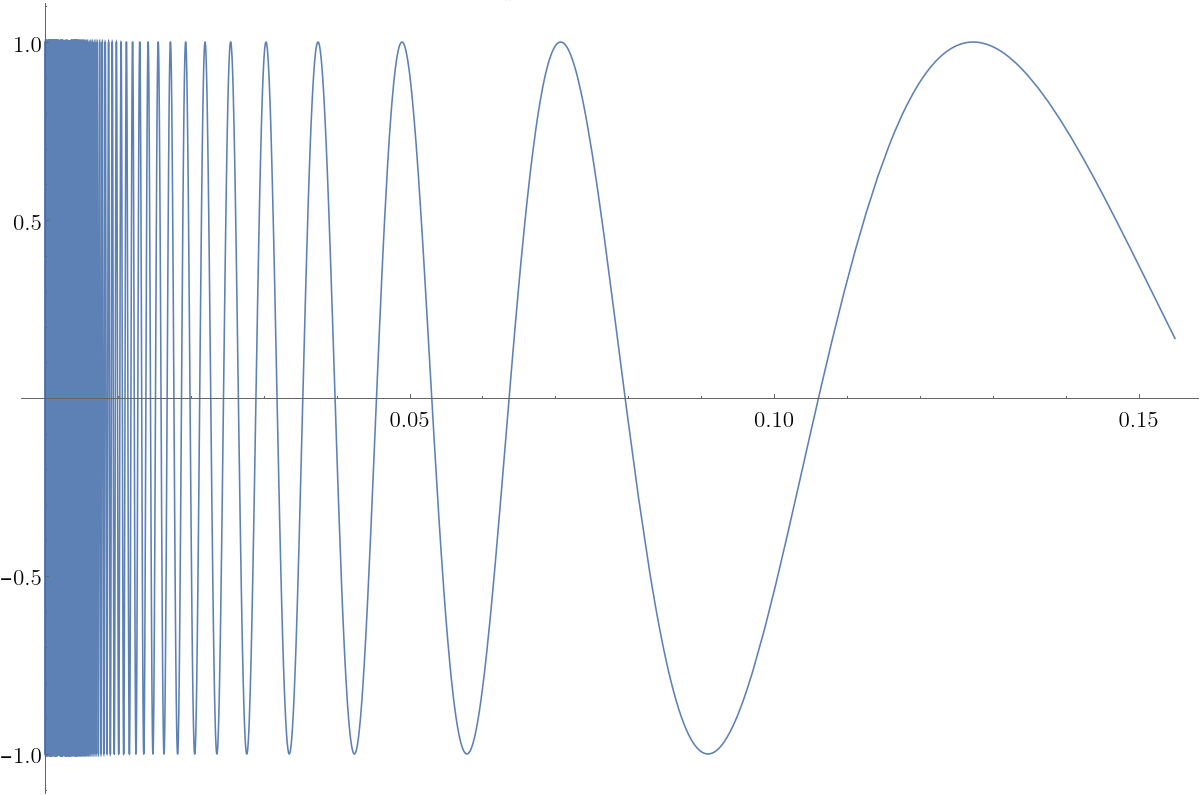
\includegraphics[width=0.5\textwidth]{figs/Topologists_Sine_Curve}
    \caption{The Topologist's Sine Curve}\label{fig:topologists_sine_curve}
  \end{figure}

  Clearly $S$ is arcwise connected and thus connected.
  This is because $\sin\pqty{\frac{1}{x}}$ is continuous and so we can just parameterize along the path.

  Consider the set
  \[
    T = (\set{0} \times [-1, 1]) \sqcup \Set{\pqty{x, \sin\pqty{\frac{1}{x}}} | 0 < x \leq 1 } \subseteq \R^{2}.
  \]
  We will show this path is connected but not arcwise connected.
  The intuition here is that we cannot ``get to'' a portion of the $y$-axis in finite time starting from a point on the sine curve due to the rapid oscillation.

  We claim that $\overline{S} = T$.
  Note that the function $\sin\pqty{\frac{1}{x}}$ is continuous for all $x > 0$ and so every point on it is a limit point.
  Now consider a point $(0, y)$ where $y \in [-1, 1]$.
  Then due to the rapid oscillation of $\sin\pqty{\frac{1}{x}}$ as $x \to 0$ we have that every open ball around $(0, y)$ has non-trivial intersection with the curve infinitely often and so $(0, y)$ is a limit point of some sequence of points in $S$.
  Thus every point in $T$ is a limit point of some sequence of points in $S$ and $T \subseteq \overline{S}$.

  To show that $\overline{S} \subseteq T$ it suffices to show that $T$ is closed since $S \subseteq T$.
  Closed sets contain their limit points so let $\set{(x_{n}, y_{n})}$ be a sequence of points in $T$ with limit $(x, y)$.
  We know that $x = \lim x_{n}$ and $y = \lim y_{n}$ so $x \geq 0$ and $y \in [-1, 1]$.
  If $x = 0$ then we are done since $(0, y) \in T$ for $y \in [-1, 1]$.
  So now suppose $x > 0$ and we can assume that after dropping some number of starting terms $x_{n} > 0$ for all $n$.
  Thus $(x_{n}, y_{n})$ lies on the curve $\sin\pqty{\frac{1}{x}}$.
  Since this function is continuous we get that $(x, y)$ lies on the curve and thus $T$ is closed.
  Thus $\overline{S} \subseteq T$ and overall we have equality.

\clearpage

  Note that since $S$ is connected, since it is arcwise connected, we have that $T$ is also connected by \Cref{lem: closure_of_connected_is_connected}. We now show that $T$ is not path-connected.
  Suppose that we have some path $\lambda$ connecting a point $\lambda(0) = p$ on the sine curve to $\lambda(1) = (0, 1)$.
  Let $\e = \frac{1}{2}$.
  By continuity of $\lambda$ there is some $\delta > 0$ such that $\abs{\lambda(t) - (0, 1)} < \frac{1}{2}$ for $t \in [1 - \delta, 1]$.
  The sine curve keeps escaping the disc of radius $\frac{1}{2}$ around $(0, 1)$.
  In particular this means that we cannot have continuity since the curve will eventually be of distance $> \frac{1}{2}$ from $(0, 1)$.
  Thus $T$ is not path-connected.
\end{ex}

\clearpage

\subsection*{Exercises}

\begin{exercise}[\tcite{book:Bredon} 1.4.1]
  If $A$ is a connected subset of a topological space $X$ and $A \subseteq B \subseteq \overline{A}$ then $B$ is connected.
\end{exercise}
\begin{pf}
  Suppose $U, V$ are a separation of $B$.
  Then note that $A = (U \cap A) \sqcup (V \cap A)$.
  But $U \cap A$ and $V \cap A$ are open in $A$ and since $A$ is connected we have that one of these, say $U \cap A$, is empty.
  Thus $A \subseteq X \setminus U$ which is closed.
  This means that $\overline{A} \subseteq X \setminus U$.
  So overall now we have $U \subseteq B \subseteq \overline{A} \subseteq X \setminus U$.
  This can hold if and only if $U$ is empty.
  Thus $B$ is connected.
\end{pf}

\begin{defn}[Locally Connected Space]
  A topological space $X$ is \emph{locally connected} if for each $x \in X$ and each neighborhood $N$ of $x$, there is a connected neighborhood $V$ of $x$ such that $V \subseteq N$.
\end{defn}

\begin{exercise}[\tcite{book:Bredon} 1.4.2]
  If $X$ is locally connected, then its components are open and equal to its quasi-components.
\end{exercise}
\begin{pf}
  Let $C$ be a component of $X$ and $x \in C$.
  Then $X$ itself is a neighborhood of $x$ and so there is a connected neighborhood $V$ of $x$ such that $V \subseteq X$.
  $V$ is connected so $V \subseteq C$.
  Since $V$ is a neighborhood of $x$, there exists an open $U \subseteq V$ such that $x \in U \subseteq C$.
  Thus $C$ is open.

  We already know that components are contained in quasi-components.
  Let $C$ be a component and $Q$ the quasi-component containing $C$ and suppose $C \subsetneq Q$.
  $C$ is open and we know that components are also closed and so $C$ is clopen in $X$.
  Let $x \in C$ and $y \in Q \setminus C$.
  Then $X = C \sqcup (Q \setminus C)$ is a separation of $X$.
  Thus there exists a DVM $d$ such that $d(x) \neq d(y)$ meaning that $x$ and $y$ are in different quasi-components.
  But $x \in C \subseteq Q$ and $y \in Q \setminus C \subseteq Q$ which is a contradiction and so $C = Q$.
\end{pf}

\begin{exercise}[\tcite{book:Bredon} 1.4.3]\label{exercise:unit_interval_connected}
  The unit interval $[0, 1]$ is connected.
\end{exercise}
\begin{pf}
  Suppose that $U, V$ formed a separation of $x$ such that $1 \in V$.
  Let $x = \sup(U) \in [0, 1]$ since the unit interval is closed.
  Suppose $x \in U$, then since $U$ is open there exists $\e > 0$ such that $B_{\e}(x) \subseteq U$ meaning that $x + \frac{\e}{2} \in U$ which is a contradiction to our choice of $x$.
  Thus $x \in V$ which is also open meaning there exists $\e > 0$ such that $B_{\e}(x) \subseteq V$.
  Thus $x - \frac{\e}{2} \in V$.
  Suppose that $x - \frac{\e}{2}$ is not an upper bound for $U$.
  Then there is some $p \in U$ such that $p > x - \frac{\e}{2}$.
  Thus $p \in \pqty{\frac{x - \e}{2}, x} \subseteq B_{\e}(x) \subseteq V$ and so $p \in V$ contradicting the disjointness of $U$ and $V$.
  Thus $x - \frac{\e}{2}$ is a lower upper bound of $U$ than $x = \sup(U)$ which is a contradiction.
  Thus we have found $x \in [0, 1]$ such that $x \notin U$ and $x \notin V$ which is a contradiction as well and $[0, 1]$ is connected.
\end{pf}

\clearpage

\chapter{Separation Axioms}

\begin{defn}[Separation Axioms, Hausdorff, Regular, Normal Spaces]
  The \emph{Separation Axioms}:
  \begin{itemize}
  \item[(T$_{0}$)] A topological space $X$ is called a \emph{T$_{0}$-space} if for any two points $x \neq y$ there is an open set containing one of them but not the other.
                   This says that point can be distinguished by the open sets where they lie.
  \item[(T$_{1}$)] A topological space $X$ is called a \emph{T$_{1}$-space} if for any two points $x \neq y$ there is an open set containing $x$ but not $y$ and another open set containing $y$ but not $x$.
        This says that singletons, and thus finite sets, are closed.
        Let $x \in X$.
        For each point $y \neq x$ let $U_{y}$ be an open set containing $y$ but not $x$.
        Then $X \setminus \set{x} = \bigcup_{y} U_{y}$ which is open and thus $\set{x}$ is closed.
        Conversely if $\set{x}$ is closed, then $X \setminus \set{x}$ is open and contains the other point.
  \item[(T$_{2}$)] A topological space $X$ is called a \emph{T$_{2}$-space} or \emph{Hausdorff} if for any two points $x \neq y$ there are disjoint open sets $U$, $V$ with $x \in U$ and $y \in V$.
        This is the most useful type of space.
        It essential means that ``limits'' are unique.
  \item[(T$_{3}$)] A T$_{1}$-space $X$ is called a \emph{T$_{4}$-space} of \emph{regular} if for any point $x$ and closed set $F$ not containing $x$ there are disjoint open sets $U$, $V$ with $x \in U$ and $F \subseteq V$.
  \item[(T$_{4}$)] A T$_{1}$-space $X$ is called a \emph{T$_{5}$-space} of \emph{normal} if for any two disjoint closed sets $F$, $G$ there are disjoint open sets $U$, $V$ with $F \subseteq U$ and $G \subseteq V$.
  \end{itemize}
\end{defn}

\begin{ex}[A Space that is not  $T_0$]
  The topology on $\set{x, y}$ where the only open sets are $\emptyset$ and $\set{x, y}$ is not $T_{0}$.
  There is no open set containing $x$ and not $y$ nor vice versa.
\end{ex}

\begin{ex}[A Space that is $T_0$ but not $T_1$]
  The topology on $\set{x, y}$ with open sets $\emptyset, \set{x}$, and $\set{x, y}$ is $T_{0}$.
  This is because $\set{x}$ is an open set containing $x$ but not $y$.
  However, there is no open set containing $y$ but not $x$ so the space is not $T_{1}$.
\end{ex}

\clearpage

\begin{prop}\label{prop: regular_iff_closed_neighborhood_basis}
  A Hausdorff space $X$ is regular if and only if the closed neighborhoods of any point form a neighborhood basis of the point.
\end{prop}
\begin{pf}
  Suppose $X$ is regular.
  Let $x \in V$ for $V$ open and let $C \defeq X \setminus V$.
  Then by regularity there exist open sets $U$ and $W$ with $x \in U$, $C \subseteq W$, and $U \cap W = \emptyset$.
  Then $X \setminus W$ is closed and $X \setminus W \subseteq X \setminus C = V$ and so any neighborhood of $V$ of $x$ contains a closed neighborhood of $x$.

  Now suppose that every point has a closed neighborhood basis.
  Let $x \in C$ with $C$ closed and $V = X \setminus C$.
  Then there exists open $U$ with $\overline{U} \subseteq V = X \setminus C$ and $x \in U$.
  Then $C \subseteq X \setminus \overline{U}$ and $U \cap (X \setminus \overline{U}) = \emptyset$.
  Thus $X$ is regular.
\end{pf}

\begin{cor}
  A subspace of a regular space $X$ is regular.
\end{cor}
\begin{pf}
  If $A \subseteq X$ is a subspace, just intersect a closed neighborhood basis in $X$ of some $a \in A$ with $A$ to obtain a closed neighborhood basis of $a$ in A.
\end{pf}

\clearpage

\subsection*{Exercises}

\begin{exercise}[\tcite{book:Bredon} 1.5.2]
  A finite $T_{1}$-space is discrete.
\end{exercise}
\begin{pf}
  Let $X$ be a finite $T_{1}$ space and $x \in X$.
  For all $y \neq x$ we can find an open set $U_{y}$ such that $y \notin U_{y}$ but $x \in U_{y}$.
  Then $\set{x} = \bigcap_{y \neq x} U_{y}$ is open since it is a finite intersection.
  Thus since singletons are open, their unions are open.
  This means arbitrary subsets of $X$ are open and we have the discrete topology.
\end{pf}

\begin{exercise}[\tcite{book:Bredon} 1.5.5]\label{exercise: Bredon 1.5.5}
  Subspaces of Hausdorff Spaces are Hausdorff.
\end{exercise}
\begin{pf}
  Let $X$ be Hausdorff and $Y$ a subspace of $X$.
  Let $x \neq y$ be elements in $Y$.
  Then there exists disjoint $U, V$ open in $X$ such that $x \in U$ and $y \in V$.
  But $U \cap Y$ and $U \cap V$ are open in $Y$ and contain $x$ and $y$ respectively and are still disjoint.
  Thus $Y$ is Hausdorff.
\end{pf}

\begin{exercise}[\tcite{book:Bredon} 1.5.6]\label{exercise: bredon_1.5.6}
  A Hausdorff space $X$ is normal if and only if for all open sets $U$ and closed sets $C \subseteq U$ there is an open set $V$ with $C \subseteq V \subseteq \overline{V} \subseteq U$.
\end{exercise}
\begin{pf}
  Suppose that $X$ is normal and let $U$ open and $C$ closed in $X$ such that $C \subseteq U \subseteq X$.
  $U$ is open so $X \setminus U$ is closed and disjoint from $C$.
  Thus there exists disjoint open $V, W$ such that $C \subseteq V$ and $(X \setminus U) \subseteq W$.
  But $V \subseteq X \setminus W$ and since $X \setminus W$ is closed, it contains $\overline{V}$.
  Then we also have that $X \setminus W \subseteq U$ since $X \setminus U \subseteq W$.
  Thus overall we have $C \subseteq V \subseteq \overline{V} \subseteq X \setminus W \subseteq U$.

  Now suppose that for any $U$ open, $C$ closed such that $C \subseteq U$ we have $V$ open such that $C \subseteq V \subseteq \overline{V} \subseteq U$.
  Let $C_{1}, C_{2}$ be disjoint closed subsets of $X$.
  Since $C_{1}$ is closed, $X \setminus C_{1}$ is open and contains $C_{2}$.
  Thus there exists open $V$ such that $C_{2} \subseteq V \subseteq \overline{V} \subseteq X \setminus C_{1}$.
  $C_{2} \subseteq \overline{V}$ and $\overline{V}$ closed means that $C_{1} \subseteq X \setminus \overline{V}$ which is open.
  Thus we have open sets $V, X \setminus \overline{V}$ that are disjoint and contain $C_{1}$ and $C_{2}$ respectively meaning that $X$ is normal.
\end{pf}

\begin{exercise}[\tcite{book:Bredon} 1.5.9]
  Metric spaces are normal.
\end{exercise}
\begin{pf}
  Let $X$ be a metric space with metric $d$.
  Recall from \Cref{prop: closed_dist_inf_0} that for closed $C \subseteq X$, $x \in X$ that $d(x, C) = 0$ if and only if $x \in C$.
  Let $C_{1}, C_{2}$ be disjoint closed sets in $X$.
  Define open sets $U_{1}$, $U_{2}$ such that
  \[
    U_{1} \defeq \bigcup_{x \in C_{1}} D_{\frac{d(x, C_{2})}{3}}(x),~ U_{2} \defeq \bigcup_{x \in C_{2}} D_{\frac{d(x, C_{1})}{3}}(x).
  \]
  We have that $C_{1} \subseteq U_{1}$ and $C_{2} \subseteq U_{2}$ and $U_{1}, U_{2}$ are open and disjoint.
  Thus $X$ is normal.
\end{pf}

\clearpage

\chapter{Nets (Moore-Smith Convergence)}

Many results in metric spaces are stated in terms of sequences.
We discuss a generalization of sequences called \emph{nets}.

\begin{defn}[Directed Sets]
  A \emph{directed set} $D$ is a poset such that for all $\alpha, \beta \in D$, there exists $\tau \in D$ such that $\tau \geq \alpha$ and $\tau \geq \beta$.
\end{defn}

\begin{defn}[Net]
  A \emph{net} in a topological space $X$ is a directed set $D$ along with a function $\phi\colon D \to X$.
\end{defn}

\begin{ex}[Sequences are Nets]
  Note that $\N$ with the usual ordering is a directed set.
  Sequences are nets with $\N$ as the directed set.
\end{ex}

\begin{defn}[Frequently, Eventually]
  If $\phi\colon D \to X$ is a net in a topological space $X$ and $A \subseteq X$, we say that $\phi$ is \emph{frequently} in $A$ if for all $\alpha \in D$ there exists $\beta \geq \alpha$ such that $\phi(\beta) \in A$.
  We say that $\phi$ is \emph{eventually} in $A$ if there exists $\alpha \in D$ such that for all $\beta \geq \alpha$ we have that $\phi(\beta) \in A$.
\end{defn}

\begin{defn}[Convergence of a Net]
  A net $\phi\colon D \to X$ in a topological space $X$ is said to \emph{converge to $x \in X$} if for any neighborhood $U$ of $x$, $\phi$ is eventually in $U$.
\end{defn}

\clearpage

\begin{prop}
  A topological space $X$ is Hausdorff if and only if any two limits of a convergent net are equal.
  Thus it makes sense to speak of the limit of a convergent net.
\end{prop}
\begin{pf}
  Suppose that $X$ is Hausdorff.
  If a net $\phi$ is eventually in two sets $U$ and $V$, then it is eventually in $U \cap V$.
  Also this means that $U \cap V \neq \emptyset$.
  Thus the forward direction is immediate.

  Now suppose that $X$ is not Hausdorff and that $x \neq y \in X$ are two points which cannot be separated by open sets.
  Consider a directed whose elements are pairs of open sets $(U, V)$ with $x \in U$, $y \in V$.
  We give this directed set the ordering $(U, V) \geq (A, B)$ if and only if $(U \subseteq A) \text{ and } (V \subseteq B)$ (so smaller sets are greater).
  Let $\phi$ be a net on this directed set such that $\phi(U, V) = $ some point in $U \cap V$.

  We claim that this net converges to both $x$ and $y$.
  Let $W$ be any neighborhood of $x$.
  Take any open set $V$ containing $y$ and an open set $U$ with $x \in U \subseteq W$.
  For any $(A, B) \geq (W, V)$ we have that $\phi(A, B) \in A \cap B \subseteq U \subseteq W$.
  Thus $\phi$ is eventually in $W$ and $\phi$ converges to $x$.
  A similar argument yields that $\phi$ also converges to $y$.
\end{pf}

\begin{prop}\label{prop: continuous_iff_net_converges}
  $f\colon X \to Y$ between topological spaces is continuous if and only if for any net $\phi$ converging to $x \in X$, the net $f \circ \phi$ in $Y$ converges to $f(x)$.
\end{prop}
\begin{pf}
  Suppose that $f$ is continuous.
  Let $\phi$ be a net in $X$ converging to $x$.
  Let $V \subseteq Y$ be an open set containing $f(x)$.
  We have that $U = f^{-1}(V)$ is a neighborhood of $x$.
  $\phi$ is eventually in $U$ so $f \circ \phi$ is eventually in $V$ and thus converges to $f(x)$.

  Now suppose that $f$ is not continuous.
  Then there is some open $V \subseteq Y$ such that $K \defeq f^{-1}(V)$ is not open.
  Let $x \in K \setminus \inte(K)$.
  Consider the directed set of open neighborhoods of $x$ with the ordering $A \geq B$ if and only if $A \subseteq B$.
  Choose any neighborhood $A$ of $x$.
  Note that $A \not\subseteq K$ so let $\phi(A) = w_{A} \in A \setminus K$ be a net.
  If $N$ is a neighborhood of $x$ and $B \geq N$, so $B \subseteq N$, then $\phi(B) = w_{B} \in B \setminus K \subseteq N$ and so $\phi$ is eventually in $N$.
  Thus $\phi$ converges to $x$.
  However $(f \circ \phi)(A) \notin V$ for any $A$ and so $f \circ \phi$ is not eventually in $V$ and thus does not converge to $f(x)$.
\end{pf}

Given a net $\phi\colon D \to X$, let $x_{\alpha} \defeq \phi(\alpha)$.
It's common to notate this net as $\set{x_{\alpha}}_{\alpha \in D}$.
So the condition in \Cref{prop: continuous_iff_net_converges} can be stated as
\[
  f\colon X \to Y \text{ continuous } \iff f(\lim x_{\alpha}) = \lim f(x_{\alpha}).
\]

\begin{prop}
  if $A \subseteq X$ then $\overline{A}$ is the set of limits of nets in $A$ which converge to $X$.
\end{prop}
\begin{pf}
  If $x \in \overline{A}$ then any open neighborhood of $x$ intersects nontrivially.
  We can make a net of this set of neighborhoods ordered by inclusion and have $x_{U} \in U \cap A$.
  This clearly converges to $x$.

  Now suppose that we have a net $\set{x_{\alpha}}$ of points in $A$ which converges to a point $x \in X$.
  Then this net is eventually in any neighborhood of $x$.
  Thus any neighborhood of $x$ has nontrivial intersection with a point in $A$ and $x \in \overline{A}$.
\end{pf}

\begin{defn}[Final Functions]
  If $D$ and $D'$ are directed sets, a function $h\colon D' \to D$ is \emph{final} if for all $\delta \in D$, there exists $\delta' \in D'$ such that $\alpha' \geq \delta'$ implies $h(\alpha') \geq \delta$.
\end{defn}

\begin{defn}[Subnets]
  A \emph{subnet} of a net $\phi\colon D \to X$ is the composition of a final map $h\colon D' \to D$ to a net $\phi \circ h$.
\end{defn}

\begin{prop}
  A net $\set{x_{\alpha}}$ is frequently in each neighborhood of a given point $x \in X$ if and only if it has a subnet which converges to $x$.
\end{prop}
\begin{pf}
  Consider the set $D'$ be ordered pairs $(\alpha, U)$ where $\alpha \in D$, $U$ is a neighborhood of $x$, and $x_{\alpha} \in U$.
  Give $D'$ the ordering on $D$ and by inclusion.
  If $(\alpha, U)$ and $(\beta, V)$ are in $D'$, then since $\set{x_{\alpha}}$ is frequently in $U$ and $V$, it is frequently in $U \cap V$.
  Thus there is some $\tau \geq \alpha, \beta$ with $x_{\tau} \in U \cap V$.
  Thus $(\tau, U \cap V) \in D'$ and $(\tau, U \cap V) \geq (\alpha, U), (\beta, V)$.
  So $D'$ is directed.

  Map $D' \to D$ by $(\alpha, U) to \alpha$.
  For any $\delta \in D$, $(\delta, X) \in D'$, and $(\alpha, X) \geq (\delta, X)$ implies that $\alpha \geq \delta$.
  So this map is final and $\set{x_{\alpha, U}}$ is a subset of $\set{x_{\alpha}}$.

  Let $N$ be a neighborhood of $x$.
  Then by assumption there exists some $x_{\beta} \in N$.
  If $(\alpha, U) \geq (\beta, N)$, then $x_{\alpha, U} = x_{\alpha} \in U \subseteq N$.
  So $\set{x_{\alpha, N}}$ is eventually in $N$.

  The converse is immediate.
\end{pf}

\begin{defn}[Universal Nets]
  A net in a set $X$ is \emph{universal} if for any $A \subseteq X$, the net is either eventually in $A$ or $X \setminus A$.
\end{defn}

\begin{prop}\label{prop: composition_with_universal_is_universal}
  The composition of a universal net in $X$ with a function $f\colon X \to Y$ is a universal net in $Y$.
\end{prop}
\begin{pf}
  If $A \subseteq Y$, then the net is eventually either in $f^{-1}(A)$ or $X \setminus f^{-1}(A)$.
  But $X \setminus f^{-1}(A) = f^{-1}(Y \setminus A)$ so the composition is either in $A$ or $Y \setminus A$.
\end{pf}

\clearpage

\begin{thrm}\label{thrm: net_has_universal_subnet}
  Every net has a universal subset
\end{thrm}
\begin{pf}
  Let $\set{x_{\alpha} | \alpha \in P}$ be a net in $X$.
  Consider all collections \textbf{C} of subsets of $X$ such that
  \begin{enumerate}
  \item $A \in \textbf{C} \implies \set{x_{\alpha}}$ is frequently in $A$; and
  \item $A, B \in \textbf{C} \implies A \cap B \in \textbf{C}$.
  \end{enumerate}
  Note that $\textbf{C} = \set{X}$ is such a collection.
  Other the family of all such collections by inclusion.
  The union of any \quest{simply ordered set} of collections satisfying conditions is another such collection.
  Thus by the \quest{maximality principle} there exists a maximal such collection $\textbf{C}_{0}$.

  Let $P_{0} = \set{(A, \alpha) \in \textbf{C}_{0} \times P | x_{\alpha} \in A}$ and order it by
  \[
    (B, \beta) \geq (A, \alpha) \iff B \subseteq A \text{ and } \beta \geq \alpha.
  \]
  This makes $P_{0}$ a directed set.
  Map $(A, \alpha) \to \alpha$ which is clearly final and thus defines a subset $\set{x_{A, \alpha}}$.

  We claim this subnet is universal.
  Suppose $S$ is any subset of $X$ such that $\set{x_{A, \alpha}}$ is frequently in $S$.
  Then for any $(A, \alpha) \in P_{0}$, there exists $(B, \beta) \geq (A, \alpha)$ in $P_{0}$ with $x_{\beta} = x_{B, \beta} \in S$.
  Then $B \subseteq A$, $\beta \geq \alpha$, and $x_{\beta} \in B$.
  Thus $x_{\beta} \in S \cap B \subseteq S \cap A$.
  This means that $\set{x_\alpha}$ is frequently in $S \cap A$ for any $A \in \textbf{C}_{0}$.
  But $S$ and $S \cap A$, for $A \in \textbf{C}_{0}$, can be added to $\textbf{C}_{0}$ and these conditions still hold.
  So by maximality, $S \in \textbf{C}_{0}$.

  If $\set{x_{A, \alpha}}$ was also frequently in $X \setminus S$, then $X \setminus S \in \textbf{C}_{0}$ be a similar argument.
  Thus $S \cap (X \setminus S) = \emptyset \in \textbf{C}_{0}$.
  This contradicts the first condition.
  Thus $\set{X_{A, \alpha}}$ is not frequently in $X \setminus S$ and so it is indeed eventually in $S$.

  Overall we have that if $\set{x_{(A, \alpha)}}$ is frequently in $S$, it is eventually in $S$.
  Thus $\set{x_{A, \alpha}}$ is a universal subset.
\end{pf}

Note that here we have used the Axiom of Choice in the form of the \quest{maximality principle}.
This past theorem is in fact equal to the Axiom of Choice.

\begin{prop}
  Subnets of universal nets are universal.
\end{prop}
\begin{pf}
  Let $\set{x_{\alpha}}$ be a universal net $\phi\colon D \to X$ and $\set{x_{h(\alpha)}}$ a subnet with final $h\colon D' \to D$.
  Let $A \subseteq X$ and without loss of generality suppose that $\set{x_{\alpha}}$ is eventually in $A$.
  Then there exists $\alpha \in D$ such that for all $\beta \geq \alpha$, $x_{\beta} \in A$.
  We have that $h$ is final and so there exists $\alpha'$ such that $\beta' \geq \alpha'$ implies that $h(\beta') \geq \beta$.
  Thus the subnet is eventually in $A$.
\end{pf}

\clearpage

\subsection*{Exercises}

\begin{exercise}[\tcite{book:Bredon} 1.6.1]
  A sequence is universal if and only if it is eventually constant.
\end{exercise}
\begin{pf}
  Let $x = \set{x_{i}}_{i \in \N}$ be a sequence in a metric space with metric $d$.
  Suppose the sequence was not eventually constant.
  Then for any $i \in \N$ we can find $\e > 0$ and $j > i$ such that $x_{j} \notin B_{\e}(x_{i})$.
  Thus the sequence is not universal.

  The converse is clear.
\end{pf}

\clearpage

\chapter{Compactness}

\begin{defn}[Covering, Open Covering, Subcover]
  A \emph{covering} of a topological space $X$ is a collection of sets whose union is $X$.
  An \emph{open covering} is a covering where each set is open.
  A \emph{subcover} is a subset of a cover which is still a cover.
\end{defn}

\begin{defn}[Compact, Heine-Borel Property]
  A topological space $X$ is said to be \emph{compact} or have the \emph{Heine-Borel property} if every open covering of $X$ has a finite subcover.
\end{defn}

\begin{defn}[Finite Intersection Property]
  A collection of sets has the \emph{finite intersection property} if the intersection of any finite subcollection is empty.
\end{defn}

The following theorem is just a translation of compactness in terms of open sets to an equivalent statement of about the closed complements of those sets.

\begin{thrm}\label{thrm: compact_iff_nonempty_intersection}
  A topological space $X$ is compact if and only if for every collection of closed subsets of $X$ which has the finite intersection property, the intersection of the whole collection is nonempty.
\end{thrm}
\begin{pf}
  \quest{Trivial Proof}
\end{pf}

\begin{thrm}\label{thrm: compact_subset_Hausdorff_closed}
  If $X$ is a Hausdorff space, then any compact subset of $X$ is closed.
\end{thrm}
\begin{pf}
  Let $A \subseteq X$ be compact and suppose that $x \in X \setminus A$.
  For $a \in A$ let $a \in U_{a}$ and $x \in V_{a}$ be disjoint open sets.
  Now $A = \bigcup_{a \in A} (U_{a} \cap A)$ and so we have a cover.
  Thus by compactness of $A$, we have $a_{1}, \ldots, a_{n} \in A$ such that $A \subseteq u_{a_{1}} \cup \cdots \cup U_{a_{n}} = U$.
  But then $x \in V_{a_{1}} \cap \cdots \cap V_{a_{n}} = V$ which is open, and $U \cap V = \emptyset$.
  Thus $x \in V \subseteq X \setminus U \subseteq X \setminus A$ and $V$ is open.
  Since this holds for any $x \in X \setminus A$, we have that $X \setminus A$ is open and thus $A$ is closed.
\end{pf}

\begin{thrm}\label{thrm: image_of_compact_is_compact}
  If $X$ is compact and $f\colon X \to Y$ is continuous, then $f(X)$ is compact.
\end{thrm}
\begin{pf}
  We may as well replace $Y$ by $f(X)$ and so assume that $f$ is onto.
  For any open cover of $f(X)$, look at inverse images of the sets and apply compactness.
\end{pf}

\begin{thrm}\label{thrm: closed_subset_of_compact_is_compact}
  If $X$ is compact and $A \subseteq X$ is closed, then $A$ is compact.
\end{thrm}
\begin{pf}
  Cover $A$ with open sets in $X$, add the open set $X \setminus A$, and then apply compactness of $X$.
\end{pf}

\begin{thrm}
  Suppose that $X$ is compact, $Y$ is Hausdorff, $f\colon X \to Y$ is a continuous bijection, then $f$ is a homeomorphism.
\end{thrm}
\begin{pf}
  We need to show that $f^{-1}$ is continuous.
  This is equivalent to showing that $f$ maps closed sets to closed sets.
  But if $A \subseteq X$ is closed, then $A$ is compact by \Cref{thrm: closed_subset_of_compact_is_compact}.
  Thus $f(A)$ is compact and $f(A)$ must be closed since $A$ is Hausdorff.
\end{pf}

\begin{ex}[Closed Intervals are compact in $\R$]\label{ex: 01_compact}
  We have that $[0, 1]$ is compact in $\R$.
\end{ex}
\begin{pf}
  Let $\textbf{U}$ be an open covering of $[0, 1]$.
  Let $S = \set{s \in [0, 1] | [0, s] \text{ is covered by a finite subcollection of } \textbf{U}}$.
  Then Let $b = \sup(S)$.
  Note that $S$ takes the form $[0, b]$ or $[0, b)$.
  Suppose that $S$ takes for form $[0, b)$.
  Consider a set $U \in \textbf{U}$ containing $b$.
  $U$ must contain the interval $[a, b]$ for some $a < b$.
  But we can throw this in with the interval $[0, a]$ and obtain $[0, b]$.
  So $S$ must take the form $[0, b]$.
  Now suppose that $b < 1$.
  Then \quest{a similar argument} yields that there exists $c > b$ such that there is a finite cover of $[0, c]$ which contradicts the definition of $b$.
  Thus $b = 1$ and we have a finite cover of $[0, 1]$.
\end{pf}

Overall we have that closed intervals $[a, b]$ and their closed subsets are compact.
Also note that these closed subsets must be bounded.
So in $\R$ we have that a subset is compact if and only if it is closed and bounded.
This does not hold in arbitrary metric spaces.

\begin{thrm}
  A real-valued map on a compact space takes a maximum.
\end{thrm}
\begin{pf}
  If $f\colon X \to \R$ is a real-valued map on a compact space, then $f(X)$ is compact.
  Since $f(X)$ is compact, it is closed and bounded.
  This means that $\sup(f(X))$ exists, is finite, and belongs to $f(X)$.
\end{pf}

\begin{thrm}\label{thrm: compact_haus_is_norm}
  Compact Hausdorff spaces are normal
\end{thrm}
\begin{pf}
  Suppose that $X$ is a compact Hausdorff space.
  First we show that $X$ is regular.
  Let $C$ be a closed subset of $X$ and let $x \notin C$.
  $X$ is Hausdorff so for any $y \in C$ there exists open disjoint $U_{y}$, $V_{y}$ such that $x \in U_{y}$ and $y \in V_{y}$.
  $C$ is closed and so it is compact by \Cref{thrm: closed_subset_of_compact_is_compact}.
  $V_{y}$ is an open cover of $C$ and so there exist $y_{1}, \ldots, y_{n}$ such that $C \subseteq V \defeq V_{y_{1}} \cup \cdots \cup V_{y_{n}}$.
  Let $U \defeq U_{y_{1}} \cap \cdots \cap U_{y_{n}}$.
  Then we have that $x \in U$, $C \subseteq V$, and $U, V$ disjoint and open.
  Thus $X$ is regular.

  Now repeat this same proof letting a closed set $F$ play the role of $x$ and the other closed set $G$ playing the role of $C$.
  Thus $X$ is normal.
\end{pf}

\begin{defn}[Proper Maps]
  A map $f\colon X \to Y$ is \emph{proper} if $f^{-1}(C)$ is compact for each compact $C \subseteq Y$.
\end{defn}

\clearpage

\begin{thrm}\label{thrm: closed_single_point_preimage_compact}
  If $f\colon X \to Y$ is closed and $f^{-1}(y)$ is compact for each $y \in Y$, then $f$ is proper.
\end{thrm}
\begin{pf}
  Let $C \subseteq Y$ be compact and let $\set{U_{\alpha} | \alpha \in A}$ be an indexed collection of open sets whose union contains $f^{-1}(C)$.
  For any $y \in C$, there exists a finite subset of $A_{y} \subseteq A$ such that $f^{-1}(y) = \bigcup_{\alpha \in A_{y}} U_{\alpha}$.
  Now let
  \begin{align*}
    W_{y} &= \bigcup_{\alpha \in A_{y}} U_{\alpha}, \\
    V_{y} &= Y \setminus f(X \setminus W_{y}).
  \end{align*}
  These are both open sets.
  $f^{-1}(V_{y}) \subseteq W_{y}$ and $y \in V_{y}$.
  Since $C$ is compact and covered by $V_{y}$, there exists $y_{1}, \ldots, y_{n}$ such that $C \subseteq V_{y_{1}} \cup \cdots \cup V_{y_{n}}$.
  Thus
  \begin{align*}
    f^{-1}(C) &\subseteq f^{-1}(V_{y_{1}}) \cup \cdots \cup f^{-1}(V_{y_{n}}) \\
              &\subseteq W_{y_{1}} \cup \cdots \cup W_{y_{n}} \\
              &= \bigcup_{\substack{\alpha \in A_{y_{i}} \\ 1 \leq i \leq n}} U_{\alpha}
  \end{align*}
  which is a finite open subcover of $f^{-1}(C)$.
\end{pf}


\begin{thrm}\label{thrm: compact_iff_FIP_iff_universal_etc}
  For a topological space $X$, the following are equivalent:
  \begin{enumerate}
  \item $X$ is compact.
  \item Every collection of closed subsets of $X$ with the finite intersection property has non-empty intersection.
  \item Every universal net in $X$ converges.
  \item Every net in $X$ has a convergent subset.
  \end{enumerate}
\end{thrm}
\begin{pf}
  We have already seen the equivalence of $1$ and $2$ and now we show the rest.
  \begin{enumerate}
  \item[] $1 \iff 2$ See \Cref{thrm: compact_iff_nonempty_intersection}.
  \item[] $1 \implies 3$ Suppose that $\set{x_{\alpha}}$ is a universal net that does not converge.
        Given $x \in X$, there is an open neighborhood of $U_{x}$ such that $\set{x_{\alpha}}$ is not eventually in  $U_{x}$ and so the net is eventually in $X \setminus U_{x}$.
        So there exists $\beta_{x}$ such that for all $\alpha \geq \beta_{x}$ we have that $x_{\alpha} \notin U_{x}$.
        Now cover $X$ by some finite cover $U_{x_{1}} \cup \cdots U_{x_{n}}$.
        Let $\alpha \geq \beta_{x_{i}}$ for all $i$, then $x_{\alpha} \notin U_{x_{i}}$ for any $i$.
        Thus $x_{\alpha} \notin X$ which is a contradiction.
  \item[] $3 \implies 4$ This is clear by \Cref{thrm: net_has_universal_subnet}.

\clearpage

  \item[] $4 \implies 2$ Let $\textbf{F} = \set{C}$ be a collection of closed sets with the finite intersection property.
        Without loss of generality, we can assume that \textbf{F} is closed under finite intersection.
        Order \textbf{F} by $C \geq C'$ if and only if $C \subseteq C'$, making \textbf{F} a directed set.
        Let $\set{x_{C}}_{C \in \textbf{F}}$ be a net.
        By assumption, there is a convergent subnet given by a final map $f\colon D \to \textbf{F}$.
        Thus for $\alpha \in D$, $f(\alpha) \in \textbf{F}$ and $x_{f(\alpha)} \in f(\alpha)$.
        Suppose that $x_{f(\alpha)}$ converges to $x$.
        Let $C \in \textbf{F}$.
        Then there is $\beta \in D$ such that for all $\alpha \geq \beta$ we have $f(\alpha) \subseteq C$.
        Thus $x_{f(\alpha)} \in f(\alpha) \subseteq C$.
        Since $C$ is closed, it contains its limit points and $x \in C$ meaning that $x \in \bigcap_{C \in \textbf{F}} C$ and the total intersection is nonempty.
  \end{enumerate}
\end{pf}

\begin{prop}\label{prop: closed_cap_compact_is_compact}
  The intersection of a closed set and a compact set is compact.
\end{prop}
\begin{pf}
  Let $L$ be closed and $K$ compact.
  Suppose that $\set{x_{i}}$ is a net in $L \cap K$.
  Since $K$ is compact, by \Cref{thrm: compact_iff_FIP_iff_universal_etc} there must be some subnet converging to $x \in K$.
  But $L$ is closed, so it contains its limit points, and thus $x \in L$.
  Since every net in $K \cap L$ has a convergent subnet, $K \cap L$ must be compact.
\end{pf}

\clearpage

\subsection*{Exercises}

\begin{exercise}[\tcite{book:Bredon} 1.7.1]
  Show that if $X$ is compact, then every net in $X$ has a convergent subnet without using universal nets.
\end{exercise}
\begin{pf}
  Recall that for any collection of closed subsets of $X$ with the finite intersection property, the intersection of the whole collection has nonempty intersection.
  Let $\set{x_{\alpha}}_{\alpha \in A}$ be a net in $X$ and for each $\alpha$ let $E_{\alpha} \defeq \set{x_{\beta} | \beta \geq \alpha}$.
  Then note that the collection $\set{\overline{E_{\alpha}}}$ has the finite intersection property.
  Consider a finite intersection $\bigcap_{\alpha \in I} \overline{E_{\alpha}}$.
  Let $\alpha^{*} \geq \alpha$ for all $\alpha \in I$, which exists since $A$ is a directed set.
  Then $\alpha^{*} \in \overline{E_{\alpha}}$ for all $\alpha \in I$ and so in particular the finite intersection is non-empty.
  Thus we have that the intersection the whole collection $\bigcap_{\alpha \in A} \overline{E_{\alpha}}$ is non-empty containing some element $x \in X$.

  Consider the set $B = \set{\alpha, U_{\alpha} | \alpha \in A,~ U_{\alpha} \text{ is a neighborhood of } x_{\alpha}}$.
  This can be made directed by $(\alpha, U_{\alpha}) \geq (\beta, U_{\beta})$ if and only if $\alpha \geq \beta$ and $U_{\alpha} \subseteq U_{\beta}$.
  Consider the map $h\colon B \to A$ such that $h(\alpha, U_{\alpha}) \to \alpha$.
  This is clearly final.

  This subnet $\set{x_{(\alpha, U_{\alpha})}}$ converges to $x$.
  Let $U$ be a neighborhood of $x$.
  By construction, there exists some $\alpha$ such that $x_{\alpha} \in U$ since each of the $\overline{E_{\alpha}}$ are closed sets.
  So consider $(\alpha, U) \in B$.
  Then for all $(\beta, U_{\beta}) \geq (\alpha, U)$ we have that $h(\beta, U_{\beta}) \geq \alpha$ and thus $x_{\beta} \in U_{\beta} \subseteq U$, a convergent subnet.
\end{pf}

\begin{exercise}[\tcite{book:Bredon} 1.7.2]
  Let $X$ be a compact space and $\set{C_{\alpha} | \alpha \in A}$ a collection of closed sets which is also closed with respect to finite intersection.
  Let $C \defeq \bigcap C_{\alpha}$ and suppose that $C \subseteq U$ for some $U$ open.
  Then for some $\alpha$, we have that $C_{\alpha} \subseteq U$.
\end{exercise}
\begin{pf}
  Note that $V \defeq X \setminus U$ and $V \cap C_{\alpha}$ are both closed and thus compact.
  Also note that
  \[
    \bigcap_{\alpha \in A} V \cap C_{\alpha} = (X \setminus U) \cap \bigcap_{\alpha \in A} C_{\alpha} = (X \setminus U) \cap C = \emptyset.
  \]
  Let $F_{\alpha} \defeq X \setminus (V \cap C_{\alpha})$ which is open.
  Fix some $\beta \in A$.
  We have that $\bigcup_{\alpha \in A} F_{\alpha}$ is an open cover for $V \cap C_{\beta}$.
  This is because if $x \in V \cap C_{\beta}$, then since $\bigcap_{\alpha \in A} V \cap C_{\alpha} = \emptyset$ there is some $\alpha$ such that $x \notin V \cap C_{\alpha}$ meaning that $x \in F_{\alpha}$.
  But $V \cap C_{\beta}$ is compact, so there is some finite subcover $A' \subseteq A$ such that
  \[
    \bigcup_{\alpha \in A'} F_{\alpha} = \bigcup_{\alpha \in A'} X \setminus (V \cap C_{\alpha}) \containseq V \cap C_{\beta}.
  \]
  This implies that
  \[
    (V \cap C_{\beta}) \cap \pqty{\bigcap_{\alpha \in A'} V \cap C_{\alpha}} = V \cap \pqty{C_{\beta \cap \bigcap_{\alpha \in A'} C_{\alpha}}} = \emptyset.
  \]
  Thus we have found a finite intersection of closed sets from the collection, which itself is a member of the collection, disjoint from $X \setminus U$ meaning that is contained in $U$ as desired.
\end{pf}

\begin{exercise}[\tcite{book:Bredon} 1.7.3]
  Show that the hypothesis in \Cref{thrm: closed_single_point_preimage_compact} that $f$ is closed is necessary.
\end{exercise}
\begin{pf}
  Recall that subsets of $\R$ are compact if and only if they are closed and bounded.
  Note that $(0, 1]$ is bounded but not closed.
  This is because $\R \setminus (0, 1]$ is open, and in particular there is no open ball around $0$ completely contained in $R \setminus (0, 1]$.

  Now consider the inclusion $f\colon (0, 1] \into [0, 1]$.
  This satisfies the hypothesis that $f^{-1}(y)$ is compact for all $y \in [0, 1]$.
  Clearly $f^{-1}(0) = \emptyset$ is compact.
  We also have for $y > 0$ that because $[y, 1]$ is compact and $\set{y}$ is closed, $f^{-1}(y) = \set{y}$ is compact.
  However $f$ is not proper since $[0, 1]$ is compact but $f^{-1}([0, 1]) = (0, 1]$ is not compact.
\end{pf}

\clearpage

\chapter{Products}

\begin{defn}[Product Topology, Tychonoff Topology]
  Let $X$ and $Y$ be topological spaces.
  Then the \emph{product topology} on $X \times Y$ is the topology with the subbasis $\set{U \times V | U, V \text{ open },~ U \subseteq X,~ V \subseteq Y}$.
  Similarly, one can define a product topology on a finite product $X_{1} \times \cdots \times X_{n}$.

  For an infinite product $\Bigtimes_{\alpha \in A} X_{\alpha}$, we define the product topology as the topology with basis
  \[
    \bigtimes_{\substack{\alpha \in A \\ U_{\alpha} \subseteq X_{\alpha} \text{ open }}} U_{\alpha}
  \]
  such that $U_{\alpha} = X_{\alpha}$ for all but a finite number of $\alpha$ (``almost all $\alpha$'').
  This topology has subbasis $U_{\alpha} \times \Bigtimes_{\beta \neq \alpha} X_{\beta}$ for $U_{\alpha}$ open in $X_{\alpha}$.
  This is also known as the \emph{Tychonoff Topology}.
\end{defn}

\begin{prop}
  The projections $\pi_{X}\colon X \times Y \to X$ and $\pi_{Y}\colon X \times Y \to Y$ are continuous and the product topology is the smallest topology for which this is true.
  This also holds for infinite products.
\end{prop}
\begin{pf}
  The subbasis described is exactly the subbasis needed for continuity to hold.
\end{pf}

\begin{prop}
  The projection map $\pi_{\beta}\colon \Bigtimes_{\alpha} X_{\alpha} \to X_{\beta}$ is an open map.
\end{prop}
\begin{pf}
  It suffices to show for basis elements of $\Bigtimes_{\alpha} X_{\alpha}$.
  Let $\Bigtimes_{\alpha} U_{\alpha}$ be a basis element of the product topology.
  Then $\pi_{\beta}\pqty{\Bigtimes_{\alpha} U_{\alpha}} = U_{\beta}$ is open in $X_{\beta}$ which shows that $\pi_{\beta}$ is an open maps.
\end{pf}

\clearpage

\begin{prop}\label{prop: compact_proj_closed}
  If $X$ is compact, then the projection $\pi_{Y}\colon X \times Y \to Y$ is closed.
\end{prop}
\begin{pf}
  Let $C \subseteq X \times Y$ be closed.
  We want to show that $Y \setminus \pi_{Y}(C)$ is open.
  Let $y \notin \pi_{Y}(C)$, meaning that $(x, y) \notin C$ for all $x \in X$.
  Then for any $x \in X$, we have open sets $U_{x} \subseteq X$ and $V_{x} \subseteq Y$ such that $x \in U_{x}, y \in V_{x}$ and $(U_{x} \times V_{x}) \cap C = \emptyset$.

  Since $X$ is compact, we can find $x_{1}, ldots, x_{n} \in X$ such that $X = U_{x_{1}} \cup \cdots \cup U_{x_{n}}$.
  Let $V = V_{x_{1}} \cap \cdots \cap V_{x_{n}}$.
  Then we have
  \[
    (X \times V) \cap C = ( U_{x_{1}} \cup \cdots \cup U_{x_{n}} ) \times ( V_{x_{1}} \cap \cdots \cap V_{x_{n}} ) \cap C = \emptyset.
  \]
  Thus $y \in V \subseteq Y \setminus \pi_{Y}(C)$ where $V$ is open meaning that $\pi_{Y}(C)$ is closed.
\end{pf}

\begin{cor}\label{cor: compact_projection_proper}
  If $X$ is compact, then the projection $\pi_{Y}\colon X \times Y \to Y$ is proper.
\end{cor}
\begin{pf}
  Immediate from \Cref{thrm: closed_single_point_preimage_compact} and \Cref{prop: compact_proj_closed}.
\end{pf}

\begin{cor}\label{cor: prod_of_compact_is_compact}
  If $X$ and $Y$ are both compact, then $X \times Y$ is compact.
\end{cor}
\begin{pf}
  The projections are proper by \Cref{cor: compact_projection_proper} so we can recover finite subcovers.
\end{pf}

\begin{cor}[Tychonoff Theorem for Finite Products]\label{cor: tychonoff_finite}
  If each of the $X_{i}$ are compact, then $X_{1} \times \cdots \times X_{n}$ is compact.
\end{cor}
\begin{pf}
  Simple inductive argument from \Cref{cor: prod_of_compact_is_compact}.
\end{pf}

\begin{cor}
  Let $I = [0, 1]$.
  Then $I^{n} \subseteq \R^{n}$ is compact.
\end{cor}
\begin{pf}
  Recall that $I$ is compact by \Cref{ex: 01_compact} and apply \Cref{cor: tychonoff_finite}.
\end{pf}

\begin{cor}
  A subspace $X$ of $\R^{n}$ is compact if and only if it is closed and bounded.
\end{cor}
\begin{pf}
  Suppose that $X$ is compact and thus closed since $\R^{n}$ is Hausdorff \Cref{thrm: compact_subset_Hausdorff_closed}.
  Cover $X$ by the open balls of radius $k$ about the origin, $k = 1, 2, \ldots$.
  Then $X$ has a finite subcover which implies $X$ is bounded.

  Now suppose $X$ is closed and bounded,
  Then it is contained in some ball of radius $k$ about the origin.
  This ball is contained in $[-k, k]^{n} \subseteq \R^{n}$, which is compact by \Cref{cor: tychonoff_finite}.
  Thus $X$ is a closed subset of a compact set which is known to be compact \Cref{thrm: closed_subset_of_compact_is_compact}.
\end{pf}

\clearpage

\begin{prop}\label{prop: net_of_product_converges}
  A net in a product space $X = \Bigtimes_{\alpha} X_{\alpha}$ converges to a point $(\ldots, x_{\alpha}, \ldots)$ if and only if its composition with each projection $\pi_{\alpha}\colon X \to X_{\alpha}$ converges to $x_{\alpha}$.
\end{prop}
\begin{pf}
  Let $h\colon D \to X$ be the net in question.
  Then $\pi_{\alpha} \circ h\colon D \to X_{\alpha}$ is a net as well.
  Suppose $h$ converges to $x = (\ldots, x_{\alpha}, \ldots)$.
  Let $U_{\alpha}$ be a neighborhood of $x_{\alpha}$.
  Then $U_{\alpha} \times \Bigtimes_{\beta \neq \alpha} X_{\beta}$ is a neighborhood of $x$.
  Thus the net $h$ is eventually in this neighborhood.
  But then $\pi_{\alpha} \circ h$ is eventually in $U_{\alpha}$ and thus $\pi_{\alpha} \circ h$ is a net converging to $x_{\alpha}$.

  \quest{Converse is clear}
\end{pf}

\begin{thrm}[Tychonoff Theorem]\label{thrm: tychonoff}
  The product of an arbitrary collection of compact spaces is compact.
\end{thrm}
\begin{pf}
  Let $X = \Bigtimes_{\alpha} X_{\alpha}$ where each of the $X_{\alpha}$ are compact.
  Let $f\colon D \to X$ be a universal net in $X$.
  Then the composition $\pi_{\alpha} \circ h$ is also universal by \Cref{prop: composition_with_universal_is_universal}.
  Thus the composition converges to some $x_{\alpha}$ by \Cref{thrm: compact_iff_FIP_iff_universal_etc}.
  Thus means that the original net $f$ converges to a point $(\ldots, x_{\alpha}, \ldots)$ by \Cref{prop: net_of_product_converges}.
  Thus since every universal net in $X$ converges, by \Cref{thrm: compact_iff_FIP_iff_universal_etc} $X$ is also compact.
\end{pf}

The ease of the proof of this result is entirely due to the use of universal nets.
This usage depends on the Axiom of Choice.
In fact, \Cref{thrm: tychonoff} is equivalent to the Axiom of Choice.
However the finite case \Cref{cor: tychonoff_finite} does not depend on the Axiom of Choice.

If $X$ is a space and $A$ is a set, the product of $A$ copies of $X$ is denoted by $X^{A}$.
It can be though of as the space of functions $f\colon A \to X$.
Using this, \Cref{prop: net_of_product_converges} can be restated as follows:
\begin{prop}
  A net $\set{f_{\alpha}}$ in $X^{A}$ converges to $f \in X^{A}$ if and only if for all $x \in X$ we have that $f_{\alpha}(x) \to f(x)$.
  In particular we have that $\lim(f_{\alpha}(x)) = (\lim f_{\alpha})(x)$.
\end{prop}

When $A$ itself is also a topological space, we use $X^{A}$ to denote the set of all continuous functions $f\colon A \to X$.

\begin{prop}
  Let $X = \Bigtimes_{\alpha} X_{\alpha}$ be a product of topological spaces.
  If $X$ is normal, then each of the $X_{\alpha}$ are normal.

\end{prop}
\begin{pf}
  To see this, let $F_{\beta}, G_{\beta}$ be disjoint closed sets in $X_{\beta}$.
  Then since $\pi_{\beta}$ is continuous, we have that $\pi_{\beta}^{-1}(F_{\beta})$ and $\pi_{\beta}^{-1}(G_{\beta})$ closed.
  Thus by the normality of $X$, there exist disjoint open sets $U, V \subseteq X$ such that $\pi_{\beta}^{-1}(F_{\beta}) \subseteq U$ and $\pi_{\beta}^{-1}(G_{\beta}) \subseteq V$.
  Then since $\pi_{\beta}$ is open, we have that $\pi_{\beta}(U)$ and $\pi_{\beta}(V)$ are disjoint and open and contain $F_{\beta}$ and $G_{\beta}$ respectively.
  Thus $X_{\alpha}$ is normal.
\end{pf}

\clearpage

\begin{ex}[Sorgenfrey's Half-Open Square Topology, Product of Normal may not be Normal]\

  Let $S$ denote the real line $\R$ with the half-open topology with half-open intervals $[a, b)$ as basis elements.
  We claim that $S$ is normal.
  % TODO: redo with tikz?
  \begin{figure}[h]
    \centering
    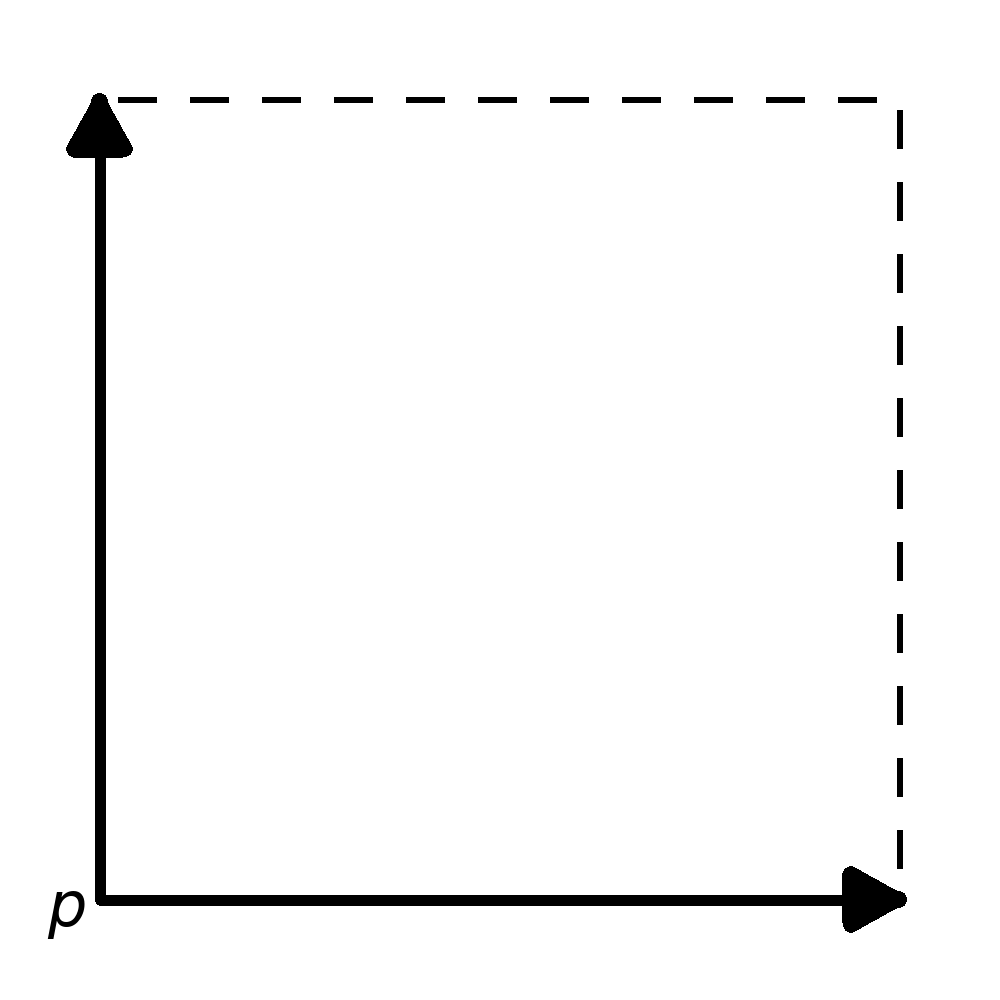
\includegraphics[width=0.25\textwidth]{figs/Sorgengrey_Half_Open.png}
    \caption{$S(p, \e)$}\label{fig:sorgenfrey_half_open}
  \end{figure}
  Let $F, G$ be disjoint closed sets in $S$.
  For each $x \in F$, choose some $x'$ such that $[x, x') \cap G$ is disjoint.
  Let $U = \bigcup_{x \in F}[x, x')$.
  We can find such $x'$ because $G$ is closed and $F$ is disjoint from $G$ and so there exists an open set around $x$ such that it is disjoint from $G$ and we can choose $x'$ from that set.
  Similarly, for each $y \in G$, choose some $y'$ such that $[y, y') \cap F$ is disjoint and let $V = \bigcup_{y \in G}[y, y')$.
  We have that $F \subseteq U$ and $G \subseteq V$.
  We also have that $U$ and $V$ are disjoint.
  To see this, it suffices to show that for all $x \in F$, $y \in G$ that $[x, x')$ and $[y, y')$ are disjoint.
  Let $x \in F$ and $y \in G$ and without loss of generality suppose $x < y$.
  Note that $x'$ was chosen such that $[x, x') \cap G = \emptyset$ and so in particular we have that $[x, x') \cap [y, y') = \emptyset$.
  Thus $x' \leq y$ which shows that $U$ and $V$ are disjoint and $S$ is normal.

  Let $X = S^{2}$ with the half-open square topology.
  Let $S(p, \e)$ denote the basis element the half-open square with sidelengths $\e$ and $p \in X$ as the lower left corner as in \Cref{fig:sorgenfrey_half_open}.
  Define $L = \set{(x, -x) | x \in \R}$.
  We have that $K = \set{(x, -x) | x \text{ is irrational }}$ is closed in $X$.
  This is because for any $(x, y) \in X \setminus K$, we have that $S((x, y), \e)$ is disjoint from $K$ for some $\e$ based on if it is above or below the line.
  If $(x, y)$ lies on the line, then since the square $S((x, y), \e)$ opens up and to the right, it is also disjoint from $K$.
  Similarly, $L \setminus K$ is closed.

  We now show that $X$ is not normal.
  \quest{Something something Baire Category Theorem, move when covered later}
\end{ex}

\clearpage

\begin{defn}[Topological Sum, Disjoint Union]
  If $X, Y$ are topological space, then their \emph{topological sum} or \emph{disjoint union} $X + Y$ is the set $(X \times \set{0}) \cup (Y \times \set{1})$ with the topology making $X \times \set{0}$ and $Y \times \set{1}$ clopen and their inclusions $X \to X + Y$ such that $x \mapsto (x, 0)$ and $Y \to X + Y$ such that $y \mapsto (y, 1)$ homeomorphisms to their image.

  More generally, if $\set{X_{\alpha} | \alpha \in A}$ is an indexed family of spaces, then their \emph{topological sum} $\bigplus_{\alpha} X_{\alpha}$ is $\bigcup_{\alpha} X_{\alpha} \times \set{\alpha}$ given the topology making each $X_{\alpha} \times \set{\alpha}$ clopen and each inclusion $X_{\beta} \to \bigplus_{\alpha} X_{\alpha}$ such that $x \to (x, \beta)$ is a homeomorphism to its image $X_{\beta} \times \set{\beta}$.
\end{defn}

In ordinary usage, if $X$ and $Y$ are disjoint space, we can regard $X + Y$ as $X \cup Y$ with the topology making $X$ and $Y$ open subspaces.

\clearpage

\subsection*{Exercises}

\begin{exercise}[\tcite{book:Bredon} 1.8.3]\label{exercise: Bredon 1.8.3}
  Let $\set{Y_{\alpha}}$ be a collection of spaces and $Y = \Bigtimes_{\alpha} Y_{\alpha}$.
  Prove that the function $f\colon X \to Y$ is continuous if and only if each composition $\pi_{\alpha} \circ f$ is continuous.
\end{exercise}
\begin{pf}
  Suppose that $f$ is continuous.
  We know the composition of two continuous functions is continuous, so $\pi_{\alpha} \circ f$ is continuous for all $\alpha$.

  Now suppose that each composition $\pi_{\alpha} \circ f$ is continuous.
  It suffices by \Cref{thrm: continuity_for_bases} to show that for each element $S$ of some subbasis \textbf{S} of $Y$, $f^{-1}(B)$ is open.
  We use the standard subbasis for the infinite product which is $U_{\alpha} \times \bigtimes_{\beta \neq \alpha} X_{\beta}$.
  We have that for any $U_{\alpha}$ that $\pqty{\pi_{\alpha} \circ f}^{-1}(U_{\alpha})$ is open by assumption.
  Thus preimages of basis elements are open and $f$ is continuous.
\end{pf}

\begin{exercise}[\tcite{book:Bredon} 1.8.4]
  An arbitrary product of Hausdorff spaces is Hausdorff and an arbitrary product of regular spaces is regular.
\end{exercise}
\begin{pf}
  Let $H = \Bigtimes_{\alpha} H_{\alpha}$ be a product of Hausdorff spaces.
  Let $x \neq y \in H$.
  Since $x \neq y$ there exists $\beta$ such that $x_{\beta} \neq y_{\beta} \in H_{\beta}$.
  Then since $H_{\beta}$ is Hausdorff let $U_{\beta}$ and $V_{\beta}$ be disjoint open sets such that $x_{\beta} \in U_{\beta}$ and $y_{\beta} \in V_{\beta}$.
  For $\alpha \neq \beta$ let $U_{\alpha} = V_{\alpha} = H_{\alpha}$.
  Let $U = \bigtimes_{\alpha} U_{\alpha}$ and $V = \bigtimes_{\alpha} V_{\alpha}$.
  We have constructed disjoint open sets $U$ and $V$ such that $x \in U$, $y \in V$ proving that $H$ is Hausdorff.

  Now let $R = \Bigtimes_{\alpha} R_{\alpha}$ be a product of regular space.
  By \Cref{prop: regular_iff_closed_neighborhood_basis}, it suffices to show that for each point $x$ in $R$, the closed neighborhoods of $x$ form a neighborhood basis of $x$.
  Let $x \in R$ and let $V$ be a neighborhood of $x$.
  Then each $V_{\alpha}$ is a neighborhood of $x_{\alpha}$ in $R_{\alpha}$ and by \Cref{prop: regular_iff_closed_neighborhood_basis} we can find $C_{\alpha}$ closed such that $x \in C_{\alpha} \subseteq R_{\alpha}$.
  Thus $C = \bigtimes_{\alpha} C_{\alpha}$ is a closed set such that $x \in C \subseteq V$ and closed neighborhoods of $x$ form a closed neighborhood basis of $x$.
  This proves that $R$ is regular.
\end{pf}

\begin{exercise}[\tcite{book:Bredon} 1.8.5]
  If $X$ is a topological space, the \emph{diagonal} of $X \times X$ is the subspace $\Delta = \set{\pqty{x, x} | x \in X}$.
  Show that $X$ is Hausdorff if and only if $\Delta$ is closed in $X \times X$.
\end{exercise}
\begin{pf}
  Suppose that $X$ is Hausdorff and let $(x, y) \in (X \times X) \setminus \Delta$.
  Then we have that there exist disjoint open sets $U_{x}, U_{y}$ such that $x \in U_{x}$ and $y \in U_{y}$.
  We have that $U_{x} \times U_{y}$ is open in $X \times X$ and contains $(x, y)$ and is contained in $(X \times X) \setminus \Delta$.
  Thus $(X \times X) \setminus \Delta$ is open meaning that $\Delta$ is closed.

  Now suppose that $\Delta$ is closed, so $(X \times X) \setminus \Delta$ is open.
  Let $x \neq y \in X$.
  Then $(x, y) \in (X \times X) \setminus \Delta$ meaning that there exists a basis element $U_{x} \times U_{y} \subseteq (X \times X) \setminus \Delta$ containing $(x, y)$.
  This implies that $U_{x} \cap U_{y} = \emptyset$.
  Thus we have found disjoint open sets $U_{x}, U_{y}$ contained in $X$ such that $x \in U_{x}$ and $y \in U_{y}$ meaning that $X$ is Hausdorff.
\end{pf}

\clearpage

\begin{exercise}[\tcite{book:Bredon} 1.8.6]
  Let $f, g\colon X \to Y$ be two maps.
  If $Y$ is Hausdorff then show that the subspace $A = \set{x \in X \mid f(x) = g(x)}$ is closed in $X$.
\end{exercise}
\begin{pf}
  Since $f$ and $g$ are continuous, we have that $h(x) = (f(x), g(x)) \subseteq Y \times Y$ is also continuous.
  Let $\Delta \subseteq Y \times Y$ be as defined in the previous problem.
  Then note that $A = h^{-1}(\Delta)$.
  Since $Y$ is Hausdorff, we have that $\Delta$ is closed which means by continuity of $h$ that $A$ is closed.
\end{pf}

\clearpage

\chapter{Metric Spaces Again}

In this section we will learn about two new concepts surrounding metric spaces.
The first will be the concept of \emph{completeness} which is a condition on sequence convergence.
The second will be about when a topological space can be equipped with a metric yielding the same open sets.

\begin{defn}[Cauchy Sequence]
  A \emph{Cauchy Sequence} in a metric space $X$ is a sequence $\set{x_{i}}_{i \in \N}$ such that for all $\e > 0$ there exists $N > 0$ such that if $n, m > N$ we have that $\dist(x_{n}, x_{m}) < \e$.
\end{defn}

\begin{defn}[Completeness]
  A metric space $X$ is \emph{complete} if every Cauchy sequence in $X$ converges in $X$.
\end{defn}

\begin{defn}[Totally Bounded]
  A metric space $X$ is \emph{totally bounded} if, for each $\e > 0$, $X$ can be covered by a finite number of $\e$ balls.
\end{defn}

Before we continue, we state an equivalent criterion for compactness in metric spaces, although it can be generalized to general topological spaces using nets.

\begin{defn}[Sequential Compactness]
  A metric space $X$ is \emph{sequentially compact} if every sequence in $X$ has a convergent subsequence.
\end{defn}

\clearpage

\begin{prop}
  A metric space $X$ is compact if and only if it is sequentially compact.
\end{prop}
\begin{pf}
  Suppose that $X$ is compact and that $x \in X$ is not the limit of a subsequence of $\set{x_{n}}$.
  Then there is an open neighborhood $U_{x}$ of $x$ containing $x_{n}$ for a finite number of $n$.
  But we can find a finite number of these $U_{x}$ that cover $X$.
  Their union would cover $X$ but only contain a finite number of the $x_{n}$ which is impossible.

  Now suppose $X$ is sequentially compact.
  First we show that $X$ is totally bounded and complete.
  Suppose that $X$ is not totally bounded.
  Then there exists $\e > 0$ such that no finite collection of $\e$-balls covers $X$.
  Let $x_{1} \in X$ and note that $B_{\e}(x_{1}) \subsetneq X$.
  Thus there exists $x_{2} \in X \setminus B_{\e}(x_{1})$ and similarly there exists $x_{e} \in X \setminus (B_{\e}(x_{1}) \cup B_{\e}(x_{2}))$.
  We can continue to iterate this construction to find a sequence of points $\set{x_{n}}_{n \in N}$.
  Then we note that for $i \neq j$ we have $\dist(x_{i}, x_{j}) > \e$ and thus we have a sequence with no convergent subsequence.
  Thus sequential compactness of $X$ implies that the set $X$ is totally bounded.
  For completeness, note that by sequential compactness any Cauchy sequence in $X$ has a convergent subsequence with limit $x \in X$.
  However using a triangle inequality argument, we can show that the whole Cauchy sequence converges to $x \in X$.
  Thus sequential compactness of $X$ implies $X$ is totally bounded and complete.

  Now suppose that $X$ is totally bounded and complete.
  Let $\set{U_{i}}_{i \in I}$ be an open cover for $X$ and for the sake of contradiction suppose it has no finite subcover.
  Then for each $N \geq 1$ we have that $X$ is covered by finitely many open balls $B_{1 / N}(x)$ for some finite set of $\set{x_{N_{i}}}$.
  We have that the $\set{U_{i}}$ has no finite subcover but finitely many open balls $B_{1 / N}(x)$ for $x \in \set{x_{N_{i}}}$ do cover $X$.
  Thus there exists some $x_{0} \in \set{x_{0_{i}}}$ such that $B_{1}(x_{0})$ is not covered by any finite subcollection of the $\set{U_{i}}$.
  If no such $x_{0}$ exists, we could find a finite subcover which would be a contradiction.
  Now we can cover $B_{1}(x_{0})$ by balls of radius $\frac{1}{2}$ such that their centers are of distance less than $1 + \frac{1}{2}$ from $x_{0}$.
  Similarly, some $x_{1}$ exists such that $B_{1/2}(x_{1})$ is not covered by any finite subcollection of the $\set{U_{i}}$.
  This continues on and on and we get a sequence $\set{x_{i}}_{i \in \N}$ which is Cauchy and by completeness converges to some point $x \in X$.
  We have that for some $i$ that $x \in U_{i}$.
  However we must also have by convergence of the sequence that there exists $n > 0$ such that $B_{2^{-n}}(x) \subseteq U_{i}$ which is a contradiction.
  Thus $X$ must be compact.
\end{pf}

We have actually proven in metric spaces an equivalence of 3 conditions.

\begin{cor}
  In a metric space $X$ the following are equivalent:
  \begin{enumerate}
  \item $X$ is compact;
  \item Every sequence in $X$ has a convergent subsequence; and
  \item $X$ is totally bounded and complete.
  \end{enumerate}
\end{cor}

\begin{defn}[Metrizable]
  A topological space $X$ is called \emph{metrizable} if it can be equipped with a metric such that the epsilon balls defined by that metric form a basis of $X$.
\end{defn}

\clearpage

\begin{defn}[Completely Regular, $T_{3 \frac{1}{2}}$, Tychonoff Space]\label{defn: completely_regular}
  A Hausdorff space $X$ is \emph{completely regular} or $T_{3 \frac{1}{2}}$ if, for each point $x$ and closed set $C \subset X$ with $x \notin C$, there is a map $f\colon X \to [0, 1]$ such that $f(x) = 0$ and $f(C) = \set{1}$.
\end{defn}

We can follow such a function with a map $[0, 1] \to [0, 1]$ which is $0$ on $\bqty{0, \frac{1}{2}}$ and stretches $\bqty{\frac{1}{2}, 1}$ onto $[0, 1]$.
This means the function $f$ in \Cref{defn: completely_regular} can be taken such that $f$ is $0$ on a neighborhood of $x$.
In fact, we can take $f^{-1}\pqty{\left[ 0, \frac{1}{2} \right)}$ and $f^{-1}\pqty{\left( \frac{1}{2}, 1 \right]}$ as disjoint open neighborhoods of of $x$ and $C$ respectively.

\begin{prop}\label{prop: bounded_metric_leq_1}
  Suppose $X$ is a metric space. Define:
  \[
  \dist'(x, y) = \begin{cases}
                   1           & \text{if } \dist(x, y) > 1, \\
                   \dist(x, y) & \text{if } \dist(x, y) \leq 1.
                 \end{cases}
  \]
  Then $\dist$ and $\dist'$ have the same topology on $X$.
\end{prop}
\begin{pf}
  The basis for the topology on $X$ only depends on the open $\e$-balls for small $\e$ and so we immediately have the same basis.
\end{pf}

\begin{prop}\label{prop: bounded_metrics_prod_top}
  Let $\set{X_{i}}_{i \in \N}$ be collection of metric spaces with metrics bounded by $1$ (\Cref{prop: bounded_metric_leq_1}).
  Define a metric on $\bigtimes_{i \in \N} X_{i}$ by $\dist(x, y) = \Sum_{i \in \N} = \frac{\dist(x_{i}, y_{i})}{2^{i}}$.
  Then this metric gives rise to the product topology.
\end{prop}
\begin{pf}
  Let $X$ denote the product set with the product topology and $X'$ denote the same set with the metric topology.
  To see that $X \to X'$ is continuous, by \Cref{exercise: Bredon 1.8.3} we just need to show that it's composition to each $X_{i}$ is continuous.
  However, all this projection does is decrease distance and multiply the distance by $2^{i}$ which clearly implies continuity.
  For the reverse, it suffice to show that for any point $x \in X$ the $\e$-ball around $x$ contains a neighborhood of $x$ in $X$.
  We have that
  \[
    B_{\e}(x) = \Set{y \in X' | \sum_{i} \frac{\dist(x_{i}, y_{i})}{2^{i}} < \e}.
  \]

  \clearpage

  Take $n$ such that $2^{-n} < \frac{\e}{4}$ and let $y_{i} \in X_{i}$ be such that $\dist(x_{i}, y_{i}) < \frac{\e}{2}$ for $i = 1, \ldots, n - 1$ and $\dist(x_{i}, y_{i})$ is arbitrary for $i \geq n$.
  Then we have that
  \begin{align*}
    \dist(x, y) &= \sum_{i = 1}^{n - 1} \frac{\dist(x_{i}, y_{i})}{2^{i}} + \sum_{i = n}^{\infty} \frac{\dist(x_{i}, y_{i})}{2^{i}} \\
                &< \sum_{i = 1}^{n - 1} \frac{\e}{2^{i + 1}} + \frac{\e}{4} \sum_{i = 0}^{\infty} \frac{1}{2^{i}} \\
                &< \frac{\e}{2} + \frac{\e}{2} = \e.
  \end{align*}
  Thus we have that
  \[
    x \in B_{\e/2}(x_{1}) \times \cdots \times B_{\e/2}(x_{n - 1}) \times X_{n} \times \cdot \subseteq B_{\e}(x)
  \]
  and note that the middle term is a basis element of the product topology as desired.
\end{pf}

\begin{lem}\label{lem: Hausdorff_and_comp_reg-ish_embedding}
  Suppose that $X$ is Hausdorff and that $f_{i}\colon X \to [0, 1]$ with $i = 1, 2, \ldots$ such that for any $x \in X$ and closed $C \subseteq X$ with $x \notin C$, there is an index $i$ such that $f_{i}(x) = 0$ and $f_{i}(C) = \set{1}$.
  Then define $f\colon X \to \Bigtimes_{i = 1, 2, \ldots} [0, 1]$ by $f(x) = (f_{1}(x), f_{2}(x), \ldots)$.
  Then $f$ is an embedding, \ie, a homeomorphism onto its image.
\end{lem}
\begin{pf}
  We have that $f$ is continuous by \Cref{exercise: Bredon 1.8.3}.
  We also have that $f$ is an injection but not a surjection because if $x$ and $y$ are distinct points, just take $C = \set{y}$ and apply the statement.
  Then note to show that $f^{-1}$ is continuous it suffices to show that $f$ is closed because $f^{-1}$ is continuous if and only if for all closed $C \subseteq X$ we have that $\pqty{f^{-1}}^{-1}(C) = f(C)$ is closed.
  Let $C \subseteq X$ be closed and suppose we have some sequence $\set{c_{i}} \subseteq C$ such that $f_{c_{i}} \to f(x)$.
  Then we just need to show the limit point $x$ is in $C$.
  If $x$ is not in $C$ then there exists an index $i$ such that $f_{i}(x) = 0$ but $f_{i}(C) = \set{1}$.
  This means that $1 = f_{i}(c_{n}) \to f_{i}(x) = 0$ which is impossible.
  Thus $x \in C$ and $f^{-1}$ is continuous and we have that $f$ is a homeomorphism onto its image.
\end{pf}

\begin{lem}\label{lem: second_count_comp_reg_family_F}
  Suppose that $X$ is second countable and is completely regular and let \textbf{S} be a countable basis for the open sets.
  For each pair of $U, V \in \textbf{S}$ with $\overline{U} \subseteq V$, take some $f\colon X \to [0, 1]$ which is $0$ on $U$ and $1$ on $X \setminus V$, provided such a function exists.
  Call \textbf{F} this (possibly empty) collection of maps.
  Note that \textbf{F} is also countable.
  Then for each $x \in X$ and each closed $C \subseteq X$ such that $x \notin C$, there is an $f \in \textbf{F}$ such that $f = 0$ on a neighborhood of $x$ and $f = 1$ on $C$.
\end{lem}
\begin{pf}
  Let $x$ and $C$ be as stated in the lemma.
  Since $C$ is closed, we have by definition of basis some $V \in \textbf{S}$ such that $x \in V \subseteq X \setminus C$.
  By $X$ being completely regular, we have some $g\colon X \to [0, 1]$ such that $g(x) = 0$ and $1$ on $X \setminus V$.
  Without loss of generality, as stated before, we can take $g = 0$ on some neighborhood of $x$.
  This neighborhood contains some $U \in \textbf{S}$ such that $\overline{U} \subseteq V$ \quest{why}, $f(U) = \set{0}$ and $f(X \setminus V) = \set{1}$.
  Thus by assumption, this $g$ can be replaced by some $f \in \textbf{F}$ satisfying the same properties as $g$ and satisfying the final requirements of the lemma.
\end{pf}

\begin{thrm}[Urysohn Metrization Theorem]\label{thrm: urysohn_metrization}
  If a space $X$ is second countable and completely regular, then it is metrizable.
\end{thrm}
\begin{pf}
  Construct a countable family of functions \textbf{F} satisfying \Cref{lem: second_count_comp_reg_family_F}.
  Then apply \Cref{lem: Hausdorff_and_comp_reg-ish_embedding} to get an embedding of $X$ into a countable product of unit intervals $[0, 1]$.
  Then by \Cref{prop: bounded_metrics_prod_top}, this countable product of intervals is metrizable.
  Thus $X$ is metrizable by the embedding.
\end{pf}

\begin{defn}[Diameter in A Metric Space]
  Let $X$ be a metric space and $A \subseteq X$. Then the \emph{diameter of $A$}, denoted $\diam(A)$, is $\sup\set{\dist(p, q) | p, q \in A}$.
\end{defn}

\begin{lem}[Lebesgue Lemma]\label{lem: lebesgue_lemma}
  Let $X$ be a compact metric space and let $\set{U_{\alpha}}$ be an open covering of $X$.
  Then there is $\delta > 0$ such that for all $A \subseteq X$ such that $\diam(A) < \delta$, there exists $\alpha$ such that $A \subseteq U_{\alpha}$.
\end{lem}
\begin{pf}
  For each $x \in X$, there exists some $\e(x) > 0$ such that $B_{2\e(x)}(x) \subseteq U_{\alpha}$ for some $\alpha$.
  Then $X$ is covered by a finite number of the balls $B_{\e(x)}$ for say $x = x_{1}, \ldots, x_{n}$.
  Let $\delta = \min_{1 \leq i \leq n} \e(x_{i})$.
  Suppose that $\diam(A) < \delta$ and pick some $a_{0} \in A$.
  There is some index $1 \leq i \leq n$ such that $\dist(a_{0}, x_{i}) < \e(x_{i})$.
  If $a \in A$ then we have that $\dist(a, a_{0}) < \delta \leq \e(x_{i})$.
  We have that $\dist(a, x_{i}) \leq \dist(a, a_{0}) + \dist(a_{0}, x_{i}) < \e(x_{i}) + \e(x_{i}) = 2\e(x_{i})$.
  Thus $A \subseteq B_{2\e(x_{i})}(x_{i}) \subseteq U_{\alpha}$ for some $\alpha$.
\end{pf}

\begin{defn}[Lebesgue Number]
  The $\delta$ in \Cref{lem: lebesgue_lemma} is called a \emph{Lebesgue Number}.
\end{defn}

\clearpage

\subsection*{Exercises}

\begin{exercise}[\tcite{book:Bredon} 1.9.2]
  A subspace of a completely regular space is completely regular
\end{exercise}
\begin{pf}
  Let $X$ be a completely regular space and $S \subseteq X$ a subspace.
  Note that by \Cref{exercise: Bredon 1.5.5} we have that $S$ is Hausdorff.
  Let $x \in S$ and $C \subseteq S$ be closed such that $x \notin C$.
  Since $C$ is closed in $S$, we have that $C = S \cap D$ for some $D$ closed in $X$.
  Also note that we must have that $x \notin D$ since $C = S \cap D$ and $x \notin C$ but $x \in S$.
  Thus by the fact that $X$ is completely regular, we have that there exists some map $f\colon X \to [0, 1]$ such that $f(x) = 0$ and $f(D) = \set{1}$.
  We can restrict $f$ to $S$ and get a map $f\mid_{S}\colon X \to [0, 1]$ such that $f\mid_{S}(0) = x$ and $f\mid_{S}(C) = f\mid_{S}(D \cap S) = f(D) = \set{1}$ as desired.
  Thus $S$ is completely regular.
\end{pf}

\clearpage

\chapter{Existence of Real Valued Functions}

In \Cref{thrm: urysohn_metrization} we relied on the fact that some set of continuous real-valued functions of sufficiently large size existed.
We now address purely topological assumptions that guarantee such functions.

\begin{lem}\label{lem: dyadic_lem_for_urysohn}
  Suppose that on a topological space $X$ we are given, for each dyadic rational number $r = \frac{m}{2^n}$ where $0 \leq m \leq 2^{m}$, an open set $U_{r}$ such that $r < s \implies \overline{U_{r}} \subseteq U_{s}$.
  Then the function
  \begin{align*}
    f\colon X &\to \R \\
      x &\mapsto
          \begin{cases}
            \inf\set{r | x \in U_{r}} & x \in U_{1} \\
            1                         & x \notin U_{1}
          \end{cases}
  \end{align*}
  is continuous.
\end{lem}
\begin{pf}
  Note that for $r$ dyadic we have
  \begin{align*}
    f(x) <    r \implies    x \in U_{r}, && \text{ hence } &&  &f(x) \geq r \impliedby x \notin U_{r}, \\
    f(x) \leq r \impliedby  x \in U_{r}, && \text{ hence } &&  &f(x) > r \implies      x \notin U_{r} \implies x \in X \setminus U_{r}.
  \end{align*}
  Thus for $\alpha$ real we have
  \[
    f^{-1}(-\infty, \alpha) = \set{x | f(x) < \alpha} = \bigcup_{r < \alpha} U_{r}
  \]
  which is open, and for $\beta$ real we have
  \[
    f^{-1}(\beta, \infty) = \set{x | f(x) > \beta} = \bigcup_{r > \beta} X \setminus U_{r} = \bigcup_{s > \beta} X \setminus \overline{U_{s}}
  \]
  which is also open.
  These half open intervals form a subbasis for $\R$ and thus $f$ is continuous.
\end{pf}

\begin{lem}[Urysohn's Lemma]\label{lem: urysohn_lemma}
  If $X$ is normal and $F \subseteq U$ where $F$ is closed and $U$ is open, then there is a map $f\colon X \to [0, 1]$ which is $0$ on $F$ and $1$ on $X \setminus U$.
\end{lem}
\begin{pf}
  Let $U_{1} = U$ and use normality of $X$ to find $U_{0}$ such that $F \subseteq U_{0} \subseteq \overline{U_{0}} \subseteq U_{1}$.
  We can do this by \Cref{exercise: bredon_1.5.6}.
  We can iterate this to find $U_{1/2}$ such that $\overline{U_{0}} \subseteq U_{1/2} \subseteq \overline{U_{1/2}} \subseteq U_{1}$.
  We also find $U_{1/4}$ such that $\overline{U_{0}} \subseteq U_{1/4} \subseteq \overline{U_{1/4}} \subseteq U_{1/2}$ and $U_{3/4}$ such that $\overline{U_{1/2}} \subseteq U_{3/4} \subseteq \overline{U_{3/4}} \subseteq U_{1}$.
  Iterate this construction repeatedly and apply \Cref{lem: dyadic_lem_for_urysohn}.
\end{pf}

\begin{cor}
  Normality implies Complete Regularity. $\qed$
\end{cor}

\begin{thrm}[Tietze Extension Theorem]
  Let $X$ be normal and $F \subseteq X$ closed and let $f\colon F \to \R$ be continuous.
  Then there is a map $g\colon X \to \R$ such that $g(x) = f(x)$ for all $x \in F$.
  Moreover, it can be arranged that
  \[
    \sup_{x \in F} f(x) = \sup_{x \in X} g(x) \text{ and } \inf_{x \in F} f(x) = \inf_{x \in X} g(x).
  \]
\end{thrm}
\begin{pf}
  First we consider the case that $f$ is bounded.
  Without loss of generality, suppose that $0 \leq f(x) \leq 1$ with infimum $0$ and supremum $1$.
  By \Cref{lem: urysohn_lemma} and the fact that $[0, 1]$ is homeomorphic to $\bqty{0, \frac{1}{3}}$, there exists a function $g_{1}\colon X \to \bqty{0, \frac{1}{3}}$ such that
  \[
    g_{1}(x) = \begin{cases}
                 0           & \text{ if } x \in F \text{ and } f(x) \leq \frac{1}{3}, \\
                 \frac{1}{3} & \text{ if } x \in F \text{ and } f(x) \geq \frac{2}{3}.
               \end{cases}
  \]
  This can be done by taking the closed set as $F \cap f^{-1}\pqty{\left(-\infty, \frac{1}{3}\right]}$ and the open set as $f^{-1}\pqty{\pqty{-\infty, \frac{2}{3}}}$.
  Let $f_{1} = f - g_{1}$.
  Note that $0 \leq f_{1}(x) \leq \frac{2}{3}$ for all $x \in F$.
  Then we can repeat this construction and find $g_{3}\colon X \to \bqty{0, \frac{1}{3} \cdot \frac{2}{3}}$ such that
  \[
    g_{2}(x) = \begin{cases}
                 0           & \text{ if } x \in F \text{ and } f(x) \leq \frac{1}{3} \cdot \frac{2}{3}, \\
                 \frac{1}{3} \cdot \frac{2}{3} & \text{ if } x \in F \text{ and } f(x) \geq \frac{2}{3} \cdot \frac{2}{3}.
               \end{cases}
  \]
  Let $f_{2} = f_{1} = g_{2}$ and note that $0 \leq f_{2}(x) \leq \pqty{\frac{2}{3}}^{2}$ for all $x \in F$.
  Inductively we can find $f_{n}$ with $0 \leq f_{n}(x) \leq \pqty{\frac{2}{3}}^{n}$ for $x \in F$.
  Then find $g_{n + 1}\colon X \to \bqty{0, \pqty{\frac{1}{3}} \cdot \pqty{\frac{2}{3}}^{n}}$ such that
  \[
    g_{n + 1}(x) = \begin{cases}
                 0           & \text{ if } x \in F \text{ and } f(x) \leq \frac{1}{3} \cdot \pqty{\frac{2}{3}}^{n}, \\
                 \frac{1}{3} \cdot \pqty{\frac{2}{3}}^{n} & \text{ if } x \in F \text{ and } f(x) \geq \frac{2}{3} \cdot \pqty{\frac{2}{3}}^{n}.
               \end{cases}
  \]
  Let $f_{n + 1} = f_{n} - g_{n + 1}$.

  \clearpage

  Now let $g(x) = \sum_{n = 1}^{\infty} g_{n}(x)$.
  This converges uniformly since $0 \leq g_{n}(x) \leq \pqty{\frac{1}{3}} \cdot\pqty{\frac{2}{3}}^{n - 1}$ which then implies that $g$ is continuous.
  For $x \in F$ we have that
  \begin{align*}
    f - g_{1}     &= f_{1}, \\
    f_{1} - g_{2} &= f_{2}, \\
                  &\vdots
  \end{align*}
  and by adding and cancelling we get
  \[
    f - (g_{1} + g_{2} + \cdots + g_{n}) = f_{n} \text{ and } 0 \leq f_{n} \leq \pqty{\frac{2}{3}}^{n}.
  \]
  Taking the limit yields that $g(x) = f(x)$ on $F$.
  Clearly the bounds are also correct.
  The infimum of $f$ is $0$ and the infimum of each of the $g_{n}$ is also $0$.
  The supremum of $f$ is $1$ and we have that
  \[
    \sup_{x \in X} g(x) = \sum_{n = 1}^{\infty} g_{n}(x) = \frac{1}{3} \sum_{n = 1}^{\infty} \pqty{\frac{2}{3}}^{n} = \frac{1}{3} * 3 = 1.
  \]

  We now consider the unbounded cases
  \begin{align*}
   \text{Case I:\@}   &f \text{ is unbounded in both directions}, \\
   \text{Case II:\@}  &f \text{ is bounded below by } a, \\
   \text{Case III:\@} &f \text{ is bounded above by } b.
  \end{align*}

  Let $h$ be a homeomorphism:
  \begin{align*}
    (-\infty, \infty) &\to (0, 1) &\text{ in Case I, }  \\
    [a, \infty)       &\to [0, 1) &\text{ in Case II, } \\
    (-\infty, b]      &\to (0, 1] &\text{ in Case III.\@}
  \end{align*}
  Then we have that $h \circ f$ is bounded by $0, 1$ and we can extend it to $g_{1}$.
  If we can arrange that $g_{1}(x)$ is never $0$ (respectively $1$) if $h \circ f$ is never $0$ (respectively $1$) then $g = h^{-1} \circ g_{1}$ would be defined and would extend $f$.
  Thus put
  \begin{align*}
    C &= \set{x | g_{1}(x) = 0 \text{ or 1 }} &\text{ in Case I, }  \\
    C &= \set{x | g_{1}(x) = 1 } &\text{ in Case II, } \\
    C &= \set{x | g_{1}(x) = 0 } &\text{ in Case III.\@}
  \end{align*}
  Then $C$ is closed and $C \cap F = \emptyset$.
  So there exists a function $k\colon X \to [0, 1]$ such that $k = 0$ on $C$ and $k = 1$ on $F$.
  Let $g_{2} = k \cdot g_{1} + (1 - k) \cdot \frac{1}{2}$.
  Then $g_{2}$ is always between $g_{1}$ and $\frac{1}{2}$ with $g_{2} \neq g_{1}$ on $C$.
  Also $g_{2} = g_{1} = h \circ f$ on $F$.
  \quest{Thus $g = h^{-1} \circ g_{2}$ extends $f$ in the desired manner}.
\end{pf}

\clearpage

\subsection*{Exercises}

\begin{exercise}[\tcite{book:Bredon} 10.2]
  If $F$ is a closed subspace of the normal space $X$ then any map $F \to \R^{n}$ can be extended to $X$.
\end{exercise}
\begin{pf}
  Tietze Extension but on each projection.
\end{pf}

\clearpage

\chapter{Locally Compact Spaces}

Many spaces, such as Euclidean spaces are not compact themselves but contain ``enough'' compact subspaces that are important to the properties of the spaces.
Locally Compact spaces are one such class of spaces.

\begin{defn}[Locally Compact Space]
  A topological space is \emph{locally compact} if every point has a compact neighborhood.
\end{defn}

\begin{prop}\label{prop: closed_subset_local_compact}
  Closed subsets of locally compact spaces are locally compact.
\end{prop}
\begin{pf}
  Let $X$ be locally compact and $F \subseteq X$ closed.
  Let $x \in F$.
  We have that $x \in X$ so it has a compact neighborhood $K$.
  Clearly $K \cap F$ is also a neighborhood of $x$.
  Let $\set{U_{\alpha}}$ be an open cover of $K \cap F$.
  $F$ is closed so $X \setminus F$ is open.
  We have that $\set{U_{\alpha}} \cup \set{X \setminus F}$ is an open cover for $K$ and thus has a finite subcover, set $\set{V_{\alpha}}$.
  Without loss of generality, we can discard $X \setminus F$ from $\set{V_{\alpha}}$ if it is included and thus we are left with a finite subcover of $K \cap F$.
  Thus $F$ is locally compact.
\end{pf}

However, the similar statement for open subsets is much more complicated.

\begin{lem}\label{lem: separate_point_compact_Hausdorff}
  Suppose that $X$ is Hausdorff, $K \subseteq X$ compact, and $p \in X \setminus K$.
  Then there are disjoint open sets $U, W$ such that $p \in U$ and $K \subseteq W$.
\end{lem}
\begin{pf}
  If $q \in K$, then by Hausdorffness we can find disjoint open sets $U_{q}$ and $V_{q}$ such that $p \in U_{q}$ and $q \in V_{q}$.
  Since $K$ is compact, we can find $q_{1}, \ldots, q_{n}$ such that $K \subseteq V_{q_{1}} \cup \cdots \cup V_{q_{n}}$.
  Then the sets
  \[
    U = U_{q_{1}} \cap \cdots \cap U_{q_{n}} \text{ and } W = V_{q_{1}} \cup \cdots \cup V_{q_{n}}
  \]
  satisfy the claim.
\end{pf}

\clearpage

\begin{lem}\label{lem: finite_subcollection_empty}
  If $\set{K_{\alpha}}$ is some collection of compact subsets of a Hausdorff space $X$ and $\bigcap_{\alpha} K_{\alpha} = \emptyset$ then some finite subcollection of the $\set{K_{\alpha}}$ also has empty intersection.
\end{lem}
\begin{pf}
  Let $V_{\alpha} = X \setminus K_{\alpha}$.
  Let $K_{1} \in \set{K_{\alpha}}$.
  Since no point of $K_{1}$ belongs to every $K_{\alpha}$, we have that $\set{V_{\alpha}}$ is an open cover of $K_{1}$.
  Thus $K_{1} \subseteq V_{\alpha_{1}} \cup \cdots \cup V_{\alpha_{n}}$ which implies that $K_{1} \cap K_{\alpha_{1}} \cap \cdots \cap K_{\alpha_{n}} = \emptyset$.
\end{pf}

\begin{prop}\label{prop: open_between_compact_and_open}
  If $X$ is a locally compact Hausdorff space and $K \subseteq U \subseteq X$ where $K$ is compact and $U$ is open, then there exists an open subset $V \subseteq X$ such that $K \subseteq V \subseteq \overline{V} \subseteq U$ and $\overline{V}$ is compact.
\end{prop}
\begin{pf}
  Since every point in $K$ has a neighborhood with compact closure due to the fact that closed subsets of compact sets are compact, and since $K$ is covered by the union of finitely many of these neighborhoods, we have that $K$ lies in an open set $G$ with compact closure.
  If $U = X$, then we are done by taking $V = G$.
  Otherwise, $U \subsetneq X$.
  Let $C = X \setminus U$.
  By \Cref{lem: separate_point_compact_Hausdorff}, we can separate $K$ and $p \in C$ by an open set $W_{p}$ such that $K \subseteq W_{p}$ and $p \notin \overline{W_{p}}$.
  Thus $\set{C \cap \overline{G} \cap \overline{W_{p}}}_{p \in C}$ is a collection of compact sets (by \Cref{prop: closed_cap_compact_is_compact}) with empty intersection.
  By \Cref{lem: finite_subcollection_empty}, we can find $p_{1}, \ldots, p_{n} \in C$ such that
  \[
    C \cap \overline{G} \cap \overline{W_{p_{1}}} \cap \cdots \cap \overline{W_{p_{n}}} = \emptyset.
  \]
  Now let
  \[
    V = G \cap W_{p_{1}} \cap W_{p_{n}}.
  \]
  We have that $K \subseteq V$ since $K \subseteq G$ and $K \subseteq$ each of the $W_{p_{i}}$.
  Then note that we have
  \[
    \overline{V} \subseteq \overline{G} \cap \overline{W_{p_{1}}} \cap \cdots \cap \overline{W_{p_{n}}}.
  \]
  since $C = X \setminus U$.
  We also have that $\overline{V}$ is compact.
  This is because $\overline{V}$ is contained in the intersection of a compact set $\overline{G}$ with a bunch of closed sets.
  Since this intersection is compact, $\overline{V}$ is a closed subset of a compact set which itself is compact.
\end{pf}

\begin{prop}\label{prop: open_subset_local_compact}
  Open subsets of locally compact Hausdorff spaces are locally compact.
\end{prop}
\begin{pf}
  Suppose that $X$ is locally compact and $U \subseteq X$ is open.
  Let $x \in U$.
  We have that $\set{x}$ is clearly compact.
  Then by \Cref{prop: open_between_compact_and_open} we can find open $V$ such that $\set{x} \subseteq V \subseteq \overline{V} \subseteq U$ with $\overline{V}$ compact.
  Thus $x$ has a compact neighborhood $\overline{V} \subseteq U$.
\end{pf}

\clearpage

\begin{thrm}
  If $X$ is a locally compact Hausdorff space then each neighborhood of a point $x \in X$ contains a compact neighborhood of $x$.
  That is, the compact neighborhoods of $x$ form a neighborhood basis at $x$.
  Moreover, $X$ is completely regular.
\end{thrm}
\begin{pf}
  Let $C$ be a compact neighborhood of $x$ and $U$ an arbitrary neighborhood of $x$.
  Let $V \subseteq C \cap U$ be open with $x \in V$.
  Then $\overline{V} \subseteq C$ is compact Hausdorff and therefore regular (\Cref{thrm: compact_haus_is_norm}).
  Thus there is a neighborhood $N \subseteq V$ of $x$ in $C$ which is closed in $\overline{V}$ and thus closed in $C$ since regular spaces have a closed neighborhood basis (\Cref{prop: regular_iff_closed_neighborhood_basis}).
  Since $N$ is closed in $C$, it is compact by \Cref{thrm: closed_subset_of_compact_is_compact}.
  Then since $N$ is a neighborhood of $x$ in $\overline{V}$ and $N = N \cap V$, $N$ is a neighborhood of $x$ in the open set $V$ and thus in $X$.
\end{pf}

\begin{thrm}\label{thrm: one_point_compactification}
  Let $X$ be a locally compact Hausdorff space.
  Define $X^{+} \defeq X \cup \set{\infty}$ where $\infty$ is just some point not in $X$.
  Define the open sets of $X^{+}$ to be open in $X$ or open in $X \setminus C$ where $C \subseteq X$ is compact.
  This defines a topology on $X^{+}$ which makes $X^{+}$ into a compact Hausdorff space.
  Moreover, this topology on $X^{+}$i s the only topology making $X^{+}$ a compact Hausdorff space with $X$ as a subspace.
\end{thrm}
\begin{pf}
  The whole space $X^{+}$ and $\emptyset$ are clearly open.
  Let $U = X^{+} \setminus C$ for $C \subseteq X$ compact.
  Then for $V$ open we have $U \cap V = V \setminus C$ which is open in $X$ since compact subsets of Hausdorff spaces are closed (\Cref{thrm: compact_subset_Hausdorff_closed}).
  The other cases of intersection of two open sets are trivial.

  Let $\set{U_{\alpha}}$ be a collection of open sets and $U = \bigcup_{\alpha} U_{\alpha}$.
  If all the $U_{\alpha}$ are open subsets of $X$ the result is immediate.
  Suppose some $U_{\beta} = X^{+} \setminus C$ where $C \subseteq X$ is compact.
  Then
  \[
    X^{+} \setminus U = \bigcap_{\alpha} X^{+} \setminus U_{\alpha} = C \cap \pqty{\bigcap_{\alpha \neq \beta} X \setminus U_{\alpha}}
  \]
  which is closed in $C$ and thus compact.
  Therefore $X^{+} \setminus U$ is closed and $U$ is open and we have a well defined topology.

  Suppose that $\set{U_{\alpha}}$ is an open cover of $X^{+}$.
  One of these sets, say $U_{\beta}$, contains $\infty$.
  $X \setminus U_{\beta}$ is closed and thus compact and has a finite subcover.
  Adding $U_{\beta}$ to this finite subcover yields a finite subcover of $X^{+}$.

  To show that $X^{+}$ is Hausdorff we just need to separate $\infty$ from any $x \in X$.
  Let $V$ be an open neighborhood of $x$ in $X$ such that $\overline{V} \subseteq X$ is compact.
  Then $x \in V$ and $\infty \in X^{+} \setminus \overline{V}$ is the required separation.

  For uniqueness, let $U \subseteq X^{+}$ be an open set in some such topology.
  Then for $C = X^{+} \setminus U$ is closed and therefore compact.
  If $C \subseteq X$ then $U$ is open in the topology described in the statement.
  If $C \not\subseteq X$ then $U \subseteq X$ must be open in $X$ since $X$ is a subspace and again $U$ is open in the topology described in the open sets.
  We now show that the open sets in the topology described in the statement are open in the given topology.
  If $U$ is open in $X$, then $U = U' \cap X$ for some $U'$ open in $X^{+}$ since $X$ is a subspace.
  But $X$ is open in $X^{+}$ since singletons are closed in Hausdorff spaces.
  Thus $U = U' \cap X$ is open in $X^{+}$.
  Next if $C$ is compact in $X$ then it must be compact in $X^{+}$ and thus $C$ is closed in $X^{+}$.
  It follows that $X^{+} \setminus X$ is open in the given topology.
\end{pf}

\begin{defn}[One-Point Compactification]
  The set $X^{+}$ in \Cref{thrm: one_point_compactification} is called the \emph{one-point compactification} of $X$.
\end{defn}

Note that if $X$ itself is compact, then $\infty$ is an isolated point (clopen) in $X^{+}$ and thus $X$ is clopen in $X^{+}$.

\begin{thrm}
  Suppose that $X$ and $Y$ are locally compact Hausdorff spaces and that $f\colon X \to Y$ is continuous.
  Then $f$ is proper if and only if $f$ extends to a continuous function $f^{+}\colon X^{+} \to Y^{+}$ with $f^{+}(\infty) = \infty$.
\end{thrm}
\begin{pf}
  $f^{+}$ exists as a function so we just need to show continuity.
  Suppose that $U \subseteq Y^{+}$ is open.
  If $U \subseteq Y$ then the result is immediate.
  Otherwise, $U = Y^{+} \setminus C$ with $C \subseteq Y$ compact.
  Thus $\pqty{f^{+}}^{-1}(U) = X^{+} \setminus f^{-1}(C)$.
  Since $f$ is proper, $f^{-1}(C)$ is compact and therefore closed.
  The result follows.

  Now suppose that we have $f^{+}$ as described.
  Then we have that $\pqty{f^{+}}^{-1}(\infty) = \infty$ and thus $\pqty{f^{+}}^{-y}(Y) = X$.
  If $C \subseteq Y$ is compact then it is closed and so $f^{-1}(C)$ is closed in $X^{+}$ and hence compact and contained in $X$.
  Thus $f$ is proper.
\end{pf}

\begin{prop}
  If $f\colon X \to Y$ is a proper map between locally compact Hausdorff spaces, then $f$ is closed.
\end{prop}
\begin{pf}
  We have an extension $f^{+}\colon X^{+} \to Y^{+}$.
  If $F \subseteq X$ is closed in $X$ then $F \cup \set{\infty}$ is closed in $X^{+}$ and hence compact.
  Thus$ f^{+}(F \cup \set{\infty})$ is compact by \Cref{thrm: image_of_compact_is_compact} and hence closed by \Cref{thrm: compact_subset_Hausdorff_closed}.
  But then $f(F) = f^{+}(F \cup \set{\infty}) \cap Y$ is closed in $Y$.
\end{pf}

\begin{defn}[Locally Closed Space]
  A subspace $A$ of a topological space is said to be \emph{locally closed} if each point $a \in A$ has an open neighborhood $U_{a}$ such that $U_{a} \cap A$ is closed in $U_{a}$.
\end{defn}

\begin{prop}\label{prop: subspace_locally_closed_iff}
  A subspace $A \subseteq X$ is locally closed if and only if it has the form $A = C \cap U$ where $U$ is open in $X$ and $C$ is closed in $X$.
\end{prop}
\begin{pf}
  Let $U = \bigcup_{a \in A} U_{a}$ which is open and $C = \overline{A}$ which is closed.
  Then we have that
  \[
    C \cap U = \overline{A} \cap \bigcup_{a \in A} U_{a} = \bigcup_{a} \overline{A} \cap U_{a} = A \cap U = A.
  \]
\end{pf}

\clearpage

\begin{thrm}
  For a Hausdorff space $X$, the following are equivalent:
  \begin{enumerate}
  \item $X$ is locally compact;
  \item $X$ is a locally closed subspace of a compact Hausdorff space; and
  \item $X$ is a locally closed subspace of a locally compact Hausdorff space.
  \end{enumerate}
\end{thrm}
\begin{pf}
  If $X$ is locally compact, then it is an open subspace of its one-point compactification $X^{+}$ which is a compact Hausdorff space by \Cref{thrm: one_point_compactification}.
  Clearly $X = X^{+} \cap X$ and so by \Cref{prop: subspace_locally_closed_iff} $X$ is a locally closed subspace.
  Thus $1$ implies $2$.
  Compact implies locally compact so $2$ implies $3$ immediately.
  If $Y \containseq X$ is locally compact and $X = C \cap U$ for $C \subseteq Y$ closed and $U \subseteq Y$ open, then $C$ is locally compact by \Cref{prop: closed_subset_local_compact} and $X = C \cap U$ is open in $C$ and hence also locally compact.
  Thus $3$ implies $1$.
\end{pf}

The prior result begs the question of when a topological space $X$ can be embedded into some compact, Hausdorff space $Y$ as a subspace.
Since $Y$ is normal (\Cref{thrm: compact_haus_is_norm}), we have that $Y$ is completely regular.
Since subspaces of completely regular sets are completely regular, we must have that $X$ is completely regular.

\begin{defn}[Stone-\Cech\ compactification]
  Let $X$ be a completely regular space and \textbf{F} the set of all maps $f\colon X \to [0, 1]$.
  Then let
  \begin{align*}
    \Phi\colon X &\to [0, 1]^{\textbf{F}} = \Bigtimes_{f \in \textbf{F}} [0, 1] \\
            \Phi(x)(f) &= f(x).
  \end{align*}
  Here we are regarding an element of $[0, 1]^{\textbf{F}}$ as a function $\textbf{F} \to [0, 1]$.
  The closure of $\Phi(X)$ is the \emph{Stone-\Cech\ compactification} of $X$ and is denoted $\beta(X)$.
\end{defn}

\clearpage

\begin{thrm}
  If $X$ is a completely regular space, then $\beta(X)$ is compact Hausdorff and $\Phi(X) \to \beta(X)$ is an embedding.
\end{thrm}
\begin{pf}
  The function $\Phi$ is one-to-one since if $\Phi(x) = \Phi(y)$ then $f(x) = f(y)$ for all $f\colon: X \to [0, 1]$ which by complete regularity implies that $x = y$.

  To prove continuity, let $\set{x_{\alpha}}$ be a net in $X$ converging to $x$.
  Then we have that
  \[
    \lim(\Phi(x_{\alpha})(f)) = \lim(f(x_{\alpha})) = f(x) = \Phi(x)(f)
  \]
  for all $f\colon X \to [0, 1]$.
  This implies that $\lim(\Phi(x)) = \Phi(x)$ by \Cref{prop: net_of_product_converges}.
  We get continuity thus by \Cref{prop: continuous_iff_net_converges}.

  For continuity of the inverse, take some net $\set{x_{\alpha}}$ in $X$ such that $\Phi(x_{\alpha})$ converges to $\Phi(x)$.
  Then for all $f\colon X \to [0, 1]$ we have
  \[
    \lim(f(x_{\alpha})) = \lim(\Phi(x_{\alpha})(f)) = \Phi(x)(f) = f(x).
  \]
  Suppose that $\set{x_{\alpha}}$ does not converge to $x$.
  Then we have some neighborhood $U$ such that $x_{\alpha}$ is frequently in $X \setminus U$.
  But some map $f\colon X \to [0, 1]$ must exist such that $f$ is $0$ at $x$ and $1$ on $X \setminus U$.
  Thus $f(x_{\alpha})$ is frequently $1$ but $f(x) = 0$ which is a contradiction to the convergence of $f(x_{\alpha})$.
\end{pf}

\begin{thrm}
  If $X$ is completely regular and $f\colon X \to\ R$ is a bounded real valued map, then $f$ can be extended uniquely to a map $\beta(X) \to \R$.
\end{thrm}
\begin{pf}
  Without loss of generality, suppose the image of $f$ is bounded between $0$ and $1$.
  Recall that $[0, 1]^{\textbf{F}}$ is the set of all functions $\textbf{F} \to [0, 1]$.
  Consider the function
  \begin{align*}
    \overline{f}\colon [0, 1]^{\textbf{F}} &\to \R \\
                \mu &\mapsto \mu(f)
  \end{align*}
  Suppose that $\set{\mu_{\alpha}}$ is a net in $[0, 1]^{\textbf{F}}$ converging to $\mu$.
  Then we have that
  \[
    \lim(\overline{f}(\mu_{\alpha})) = \lim(\mu_{\alpha}(f)) = \mu(f) = \overline{f}(\mu),
  \]
  which shows that $\overline{f}$ is continuous.
  If $x \in X$ then we have that $\overline{f}(\Phi(x)) = \Phi(x)(f) = f(x)$ which shows that $\overline{f}$ does extend $f$.
\end{pf}

\clearpage

\begin{lem}
  Let $A \subseteq X$ and $f\colon A \into Z$ be a map into a Hausdorff space $Z$.
  Then there is at most one extension of $f$ into a map $\overline{f}\colon \overline{A} \to Z$.
\end{lem}
\begin{pf}
  Suppose $\overline{f}, \overline{f}'\colon \overline{A} \to Z$ are two different such extensions of $f$.
  Then choose $x$ such that $\overline{f}(x) \neq \overline{f}'(x)$.
  Then by Hausdorffness of $Z$ there exists disjoint open neighborhoods $U$ and $U'$ such that $\overline{f}(x) \in U$ and $\overline{f}' \in U'$.
  Choose a neighborhood $V$ of $x$ such that $\overline{f}(V) \subseteq U, \overline{f}'(V) \subseteq U'$.
  By characterization of closure, $V$ intersects $A$ and this intersection contains some $y \in A \cap V$.
  Thus $\overline{f}(y) \in U, \overline{f}'(y) \in U'$.
  However by extension we have that $\overline{f}(y) = f(y) = \overline{f}'(y)$ contradicting disjointness of $U$ and $U'$.
\end{pf}

\begin{prop}
  Let $X$ be a completely regular space and $C$ a compact Hausdorff space.
  The Stone-\Cech\ compactification $\beta(X)$ satisfies the following universal property.
  If $f\colon X \to C$ is any compactification then there exists a unique map $g\colon\beta(X) \to C$ such that the following diagram commutes:
  \begin{figure}[h]
    \centering
    % https://q.uiver.app/#q=WzAsMyxbMCwwLCJYIl0sWzIsMCwiXFxiZXRhKFgpIl0sWzIsMiwiQyJdLFswLDFdLFsxLDIsIlxcZXhpc3RzIX5nIiwwLHsic3R5bGUiOnsiYm9keSI6eyJuYW1lIjoiZGFzaGVkIn19fV0sWzAsMiwiZiIsMl1d
    \[
      \begin{tikzcd}[every label/.append style={font=\normalsize}]
        X && {\beta(X)} \\
        \\
        && C
        \arrow[from=1-1, to=1-3]
        \arrow["{\exists!~g}", dashed, from=1-3, to=3-3]
        \arrow["f"', from=1-1, to=3-3]
      \end{tikzcd}
    \]
    \caption{The universal property of the Stone\Cech\ Compatification}\label{fig:stone-cech-univ}
  \end{figure}
\end{prop}
\begin{pf}
  Note that compact spaces are immediately locally compact \quest{and locally compact spaces are completely regular} so $C$ is completely regular.
  By \Cref{lem: Hausdorff_and_comp_reg-ish_embedding} we have that $C$ can be embedded into $[0, 1]^{J}$ for some $J$ so without loss of generality suppose that $C \subseteq [0, 1]^{J}$.
  Then each component function $f_{\alpha}$ of $f$ is a bounded, continuous, real-valued function of $X$.
  Thus $f_{\alpha}$ can be uniquely extended to a map $\overline{f_{\alpha}}\colon \beta(X) \to \R$.
  Define $\overline{f}\colon \beta(X) \to \R^{J}$ by $\overline{f}(x) = (\overline{f_{\alpha}}(x))_{\alpha \in J}$.
  Then $\overline{f}$ is continuous by product topology.
  In fact, we now have that $\overline{f}$ maps $\beta(X)$ into $C \subseteq \R^{J}$.
  Now let $x \in X$ and recall that $\Phi\colon X \to \beta(X)$ is the embedding of $X$ into its Stone-\Cech\ compactification.
  We have that
  \[
    \overline{f}(\Phi(x)) = (\overline{f_{\alpha}}(\Phi(x)))_{\alpha \in J} = (f_{\alpha}(x))_{\alpha \in J} = f(x)
  \]
  which shows that the diagram \Cref{fig:stone-cech-univ} commutes.
  Uniqueness is immediate by the prior lemma.
\end{pf}

\clearpage

\subsection*{Exercises}

\begin{exercise}[\tcite{book:Bredon} 1.11.1]
  Show that the Stone-\Cech\ compactification $\beta(\cdot)$ is a functor on completely regular spaces by showing that a map $f\colon X \to Y$ induces a unique commutative diagram
  \begin{figure}[h]
    \centering
    % https://q.uiver.app/#q=WzAsNCxbMCwwLCJYIl0sWzIsMCwiWSJdLFsyLDIsIlxcYmV0YShZKSJdLFswLDIsIlxcYmV0YShYKSJdLFswLDEsImYiXSxbMSwyLCJpX1kiXSxbMywyLCJcXGJldGEoZikiLDJdLFswLDMsImlfWCIsMl1d
    \[
      \begin{tikzcd}[every label/.append style={font=\normalsize}]
        X && Y \\
        \\
        {\beta(X)} && {\beta(Y)}
        \arrow["f", from=1-1, to=1-3]
        \arrow["{i_Y}", from=1-3, to=3-3]
        \arrow["{\beta(f)}"', from=3-1, to=3-3]
        \arrow["{i_X}"', from=1-1, to=3-1]
      \end{tikzcd}
    \]
    \addtocounter{figure}{1}
  \end{figure}
  such that $\beta(f \circ g) = \beta(f) \circ \beta(g)$ and $\beta(1_{X}) = 1_{\beta(X)}$.
\end{exercise}
\begin{pf}
  Suppose that $X, Y$ are completely regular spaces, $1_{X}\colon X \to \beta(X)$ and $1_{Y}\colon Y \to \beta(Y)$ their respective compactifications, and $f$ a map $X \to Y$.
  \begin{figure}[h]
    \centering
    % https://q.uiver.app/#q=WzAsMyxbMCwwLCJYIl0sWzIsMCwiXFxiZXRhKFgpIl0sWzIsMiwiXFxiZXRhKFkpIl0sWzAsMSwiaV9YIl0sWzEsMiwiXFxleGlzdHMhflxcYmV0YShmKSIsMCx7ImNvbG91ciI6WzI0MCw2MCw2MF0sInN0eWxlIjp7ImJvZHkiOnsibmFtZSI6ImRhc2hlZCJ9fX0sWzI0MCw2MCw2MCwxXV0sWzAsMiwiaV95IFxcY2lyYyBmIiwyXV0=
    \[
      \begin{tikzcd}[every label/.append style={font=\normalsize}]
        X && {\beta(X)} \\
        \\
        && {\beta(Y)}
        \arrow["{i_X}", from=1-1, to=1-3]
        \arrow["{\exists!~\beta(f)}", color={rgb,255:red,92;green,214;blue,214}, dashed, from=1-3, to=3-3]
        \arrow["{i_y \circ f}"', from=1-1, to=3-3]
      \end{tikzcd}
    \]
    \addtocounter{figure}{1}
  \end{figure}

  Since $\beta(Y)$ is compact Hausdorff, by the universal property of $\beta(X)$ we have that there exists a unique map $\beta(f)\colon \beta(X) \to \beta(Y)$ such that $\beta(f) \circ i_{X} = i_{Y} \circ f$.
  Letting $Y = X$ and $f$ be $1_{X}$ and using the fact that $1_{\beta(X)}$ is a map $\beta(X) \to \beta(X)$ yields that $\beta(1_{X}) = 1_{\beta(X)}$.

  Now let $Z$ be another completely regular space and $g$ a map $Y \to Z$.
  \begin{figure}[h]
    \centering
    % https://q.uiver.app/#q=WzAsNixbMCwwLCJYIl0sWzIsMCwiWSJdLFs0LDAsIloiXSxbMCwyLCJcXGJldGEoWCkiXSxbMiwyLCJcXGJldGEoWSkiXSxbNCwyLCJcXGJldGEoWikiXSxbMCwxLCJmIl0sWzEsMiwiZyJdLFswLDMsImlfWCIsMl0sWzEsNCwiaV9ZIiwyXSxbMiw1LCJpX1oiXSxbMyw0LCJcXGJldGEoZikiXSxbNCw1LCJcXGJldGEoZykiXSxbMyw1LCJcXGJldGEoZyBcXGNpcmMgZikiLDIseyJjdXJ2ZSI6Mn1dLFswLDIsImcgXFxjaXJjIGYiLDAseyJjdXJ2ZSI6LTJ9XV0=
    \[
      \begin{tikzcd}[every label/.append style={font=\normalsize}]
    	  X && Y && Z \\
    	  \\
    	  {\beta(X)} && {\beta(Y)} && {\beta(Z)}
    	  \arrow["f", from=1-1, to=1-3]
    	  \arrow["g", from=1-3, to=1-5]
    	  \arrow["{i_X}"', from=1-1, to=3-1]
    	  \arrow["{i_Y}"', from=1-3, to=3-3]
    	  \arrow["{i_Z}", from=1-5, to=3-5]
    	  \arrow["{\beta(f)}", from=3-1, to=3-3]
    	  \arrow["{\beta(g)}", from=3-3, to=3-5]
    	  \arrow["{\beta(g \circ f)}"', curve={height=24pt}, from=3-1, to=3-5]
    	  \arrow["{g \circ f}", curve={height=-24pt}, from=1-1, to=1-5]
      \end{tikzcd}
    \]
    \addtocounter{figure}{1}
  \end{figure}

  Then by the uniqueness of the universal property, we must have that $\beta(g) \circ \beta(f) = \beta(g \circ f)$.
\end{pf}

\clearpage
\nocite{note:conrad_topologist_sine}
\nocite{note:compactness_review}
\nocite{book:rudin_RCA}
\nocite{book:Steen_Seebach}
\nocite{book:Munkres}
\printbibliography
\end{document}
